\myChapter{Parameter adaptation in heterogeneous machines}\label{chap:adaptive}



\begin{flushright}{\slshape
    It's a wonderful thing, as a writer, to be 
    \\given parameters and walls and barriers.} \\ \medskip
    --- {Neil Gaiman}
\end{flushright}

\minitoc\mtcskip
\vfill
\lettrine{T}{he} last objective of this thesis is to apply the created framework to solve the problems previously addressed, and therefore, to be used to perform some kind of research. In this chapter, the capabilities of OSGiLiath will be used to investigate if adapting the parameters of a distributed EA taking into account the computational capabilities of the different nodes of execution leads to an increase of performance.
%FERGU: añadido el párrafo de arriba para enlazar con la tesis

This question is interesting due to new trends in distributed computing presented in Chapter \ref{chap:soa}, such as Cloud Computing, GRID
 or Service Oriented Science
 are % si se han presentado en los capítulos
                             % previos, tendrás que hacer referencia a
                             % los mismos - JJ FERGU: hecho.
leading to heterogeneous computational devices, including for instance, laptops,
tablets or desktop PCs, working in the same
environment. Thus, many laboratories, which do not count with classic
clusters but the usual workstations used by scientists, can leverage
this motley set as a heterogeneous cluster. As explained in Chapter \ref{chap:distributedEAs}, Distributed Evolutionary
Algorithms have been tested successfully in this type of systems and they have 
become very popular because their implementation is
not complex \cite{AsynchronousMultidemeMerelo08}. % Cita del asynchronous EAs del PPSN de Dortmund - JJ FERGU: hecho
Also, as presented in Chapter \ref{chap:soa}, a possible way to increase 
the interoperability within these systems is SOA, and specifically, the use of OSGiLiath framework as an example.


% frase guay, pero tienes
                                % que enganchar todo esto con LA TESIS
                                % - JJ FERGU: Hecho




%In previous chapter OSGiLiath was proposed as a framework to solve determined issues in the EA development, using a specific SOA technology. 

In this chapter, OSGiliath will be used % ¿Se podía haber usado otra
                                % cosa? ¿Esto es exclusivo de
                                % Osgiliath? - JJ FERGU: Frase al principio del capitulo
 to create a heterogeneous distributed system to be used to develop a scientific research related with parameter tuning and control (explained in Section \ref{chap:distributed:pcontroltuning}). Several services to deal with automatic binding and parameter control will be developed following SOA-EA, and deployed in different cluster configurations.






%In Section \ref{}, % where? - JJ FERGU: hecho
% we presented the work of \person{Alba \etal}, where dEAs with the same parameter
% configuration are even % cita el capítulo, no el trabajo!!! - JJ 
%more efficient in time and evaluations on heterogeneous hardware configurations than on clusters with
%homogeneous devices. % ¿en qué condiciones? ¿Siempre? Así, en general, no puede ser cierto. Un cluster de Xeons no va a ser más rápido que un Xeon y dos i5s - JJ 
%This can be explained by different reasons, such
%as different memory access times, cache sizes, or even
%implementation % ¿son más rápidos porque los tiempos de acceso a
               % memoria son diferentes? Hay que ser preciso, no vago
               % Además, ¿por qué cuentas eso? ¿Si ya se sabe, para
               % qué quieres repetirlo? ¿Estás confirmando un
               % resultado? ¿Mejorándolo? - JJ
%languages or compilers in each machine, leading to a different
%exploitation/exploration rate of the search space.  % ¿Una tasa
                                % diferentes de
                                % exploración/explotación es buena?
                                % ¿Por qué? ¡Mira mi artículo del PPSN
                                % en 2008! - JJ
%Heterogeneous parameter configuration  has also been shown to be more  efficient time-wise than a fixed
%set of parameters for different problems, as shown by \person{Gong and Fukunaga} \cite{Gong2011HeterogeneousParameters}.   


%FERGU: Comentado todo esto y arreglado párrafo arriba para justificarlo con la tesis
%These facts have motivated us to study a combination of both ideas: % esos hechos no pueden haberte motivado a estudiar nada. Tiene que haberlo hecho LA TESIS. ¿Qué tiene que ver con todo esto? - JJ
%dEAs on a heterogeneous set of nodes with different parameter values
%adapted to each node. % ¿Por qué? ¿Porque es nuevo, y por tanto mejor?
                      % ¿Porque es diferente y por tanto publicable? ¿Qué te dice que vaya a
                      % ser mejor? Y, lo más importante, ¿cómo
                      % contribuye a LA TESIS? - JJ
%In this study, the parameter to adapt to the
%computational power of each node has been the sub-population size of
%each island. % ¿Por qué? ¿Cómo? ¿Cómo se relaciona esto con LA TESIS?
             % Los capítulos deben probar LA TESIS, no decir qué se ha
             % hecho como un hecho consumado. - JJ FERGU: BORRADO TODO Y PUESTO A CONTINUACIÓN

\section{Background and problem definition}
In Section \ref{subsec:distributed:adapthetero} several works about adaptation in heterogeneous environment were presented. For example, the work of \person{Alba \etal}, where dEAs with the same parameter configuration could be more efficient in time and evaluations on heterogeneous hardware configurations than on clusters with homogeneous devices, or the work of \person{Gong and Fukunaga}, where different parameters in each island increased performance.

 These trends have motivated the usage of OSGiLiath in this chapter to give an insight to the following research questions:
\begin{itemize}
 \item Can a distributed EA be adapted to leverage the capability of a
   heterogeneous cluster?  % ¿Esa son las preguntas de la TESIS?
                           % ¿Dónde lo has dicho? - JJ FERGU: son preguntas DEL CAPÍTULO (puesto)
 \item How the adaptation of the sub-population size to the
   computational power affects the execution time and number of
   evaluations?  % Y esta pregunta es interesante porque... - JJ
 \item Is there any difference between using the same sub-population sizes in a homogeneous and a heterogeneous cluster?
 \item How is each service of the algorithm (selection, recombination, mutation, replacement and migration) affected by the different
   configurations?  % ¿Y cómo afecta todo esto a LA TESIS? - JJ
\end{itemize}

The aim of this chapter is to use OSGiLiath to demonstrate if adapting the sub-population size to the computational power of an heterogeneous cluster nodes presents an improvement in execution time. New services will be created to deal with different distributed nodes and setting the population sizes.




\subsection{Algorithm to develop}

The experimentation is centred in a distributed GA. Figure \ref{fig:EAused} shows the pseudo-code of the used algorithm. 
The algorithm is steady-state, i.e. every generation the offspring is
mixed with the parents and the worst individuals are removed. This algorithm is general enough and not designed specifically for this study.

% 1: los
                                % detalles de los EAs tendrías que
                                % haberlos dichos en su capítulo. 2:
                                % ¿Por qué SS? ¿Si no lo fuera, sería
                                % cierto? - JJ FERGU: añadida arriba
 The used neighbourhood topology for migration between islands (nodes)
 is a ring (see Figure \ref{fig:ring} in Chapter
 \ref{chap:distributedEAs}). The best individual is sent to the
 neighbour in the ring, after a fixed number of generations in each
 island. The algorithm stops when the optimum (the solution to the
 problem) is found.   % ¿Pogqué? ¿Pogqué? No puedes soltar un montón
                      % de decisiones de sopetón sin justificarlas (y
                      % sin relacionarlas con LA TESIS) - JJ FERGU: enlazado con la tesis a continuación
Therefore, a mechanism to stop all the executing nodes must be implemented.

\newsavebox{\algoadaptativebox}
\begin{lrbox}{\algoadaptativebox}
\begin{minipage}{10cm}
\begin{algorithmic} %Esto podías haberlo usado también en otros
                    %capítulos - JJ FERGU: En el unico sitio donde no lo he usado es en el del BasicGA de Eiben.
\STATE population $\gets$ initializePopulation()
\WHILE {$stop criterion not met$}
    \STATE parents $\gets$ selection(population)
    \STATE offspring $\gets$ recombination(parents)
    \STATE offspring $\gets$ mutation(offspring)
    \STATE population $\gets$ population + offspring
    \IF {time to migrate}
      \STATE migrants $\gets$ selectMigrants(population)
      \STATE remoteBuffer.send(migrants) % si haces esto, hazlo
                                % bien. ¿Dónde se declaran las
                                % variables? - JJ
    \ENDIF
    \IF {localBuffer.size $\neq$ zero}
      \STATE population $\gets$ population + localBuffer.read()
    \ENDIF
    \STATE population $\gets$ removeWorst(population)
\ENDWHILE
\end{algorithmic}
\end{minipage}
\end{lrbox}

\begin{SCfigure}[20][tb]
\usebox{\algoadaptativebox}
\caption{Pseudo-code of the used dEA: a distributed Genetic Algorithm
  (dGA).} % ¿Esto es tuyo? ¿Genérico? Si es genérico a) debería ir a
          % su capítulo b) deberías citar dónde se ha publicado - JJ
\label{fig:EAused}
\end{SCfigure}




\subsection{Problems to solve}
%No empieces con "the problems to evaluate". Di que los resultados
%deberían ser más o menos independientes del problema, pero se han
%elegido estos por tal y cual. Tienes que justificar que con estos es
%suficientes, para que no te digan el clásico "Prueba otro algoritmo"
%- JJ

The results should be independent of the problem used, but the next ones have been selected because they cover different characteristics
and computational demands. %coñe, no lo digas
                           %literlamente. ¡Justifícalo todo! ¿Qué
                           %características cubren? ¿Qué demandas
                           %computacionales? - JJ
 The problems to evaluate are the Massively Multimodal Deceptive
Problem (MMDP)  and the OneMax problem. Both problems have been described previously in Section \ref{sec:osgiliath:experiments}. Each one requires different actions/abilities by the GA
at the level of population sizing, individual selection and
building-blocks mixing \cite{AsynchronousMultidemeMerelo08}. % Podías citar los trabajos de Juanlu en esto
                        % y/o Lobo y/o Carlos Fernandes - JJ FERGU: pongo este




\subsection{Hardware and parameter configurations}

% Hala, un itemize a pelo, sin jugueteo previo ni ná de ná... ¿Por qué
% estas cuatro configuraciones? ¿Qué dificultad a priori tienen? - JJ FERGU: puesto abajo

As we are going to test parameter adaptation to hardware, different configurations should be used to compare and validate if the change in the parameters depends only of the parameters, the hardware heterogeneity, or the combination of both.

\begin{itemize}
\item HoSi/HeHa: Homogeneous Size/Heterogeneous Hardware. The same sub-population size in each island on a heterogeneous cluster.
\item HeSi/HeHa: Heterogeneous Size/Heterogeneous Hardware. Different
  sub-population sizes in each island on a heterogeneous cluster. % ¿different como? - JJ
\item HoSi/HoHa: Homogeneous Size/Homogeneous Hardware. The same
  sub-population size in each island on a homogeneous cluster. % hardware y software, ¿no? Deberías decir algo como "system" - JJ FERGU: ya, pero system puede ser también software. Prefiero dejarlo así para que quede claro todo
\item HeSi/HoHa: Heterogeneous Size/Homogeneous Hardware. Different sub-population sizes (the obtained for HeSi/HeHa) in each island on a homogeneous cluster.

\item AdSi/HeHa: Adaptive Size/Heterogeneous Hardware. Online adaptation of sub-population sizes in each island on a heterogeneous cluster.
\end{itemize} % ¿No falta AdSi HoHa? ¿Por qué no lo has puesto? - JJ FERGU: porque como la velocidad es la misma no hay cambios. Pero sí, lo pongo.



\subsection{Homogeneous Size configuration}

In this configuration, each node has 256 individuals (so, the total
amount is 1024).  % ¿Por qué? - JJ

The results of executing the algorithm in the will be used to set the sizes of the next configuration.




% ¿Ya está? ¿Nada de laxitud pos-tabla? Ahí está, y apáñatelas, ¿no? - JJ


\subsection{Heterogeneous Size configuration}

Our aim consists in validating the following hypothesis: adapting the %%%%QUITAR ESTO QUE LO HE PUESTO ARRIBA IGUAL!!!
sub-population size to the computational power of the heterogeneous
cluster nodes presents an improvement in execution time. % Hombre, ya
                                % era hora de que supiéramos la
                                % hipótesis. ¿No queríamos responder a
                                % unas preguntas? ¿Qué ha pasado con
                                % eso? ¿Cómo engancha eso con LA
                                % TESIS? - JJ
In this chapter, for a possible offline way to calculate the computational performance of each node, % ein? - JJ fERGU
 the average number of generations obtained in the
HoSi/HeHa configuration for both problems will be used to determine the
computational power of the heterogeneous machines. This comparison
takes into account all the evolutionary process in a fair manner
(proportional to the memory, processor and network usage), instead of a
traditional benchmark that usually relies only on the CPU
speed. %Hay benchmarks de todo tipo. No se puede hablar de benchmarks
       %"tradicionales" a no ser que tengas pruebas de dónde se
       %utilizan y lo cites - JJ
 %Although this is not obviously the best way, %¿Cuál es la mejor
                                %manera? ¿Por qué no la usas? - JJ FERGU: comentado
 %it is a possible
The proposed technique is a possible way to establish the computational power for the experiments of this
chapter and to determine if changing the sub-population size according
the computational power reduces the computing time of the whole
approach. %It should be considered that the contribution of this chapter
%is not the way we have computed these sizes, but compare the algorithm
%with parameters adapted to their power. % está mal escrito y aunque
                                % estuviera bien no se entiende y/o
                                % suena a excusa - JJ FERGU: lo quito, tampoco dice nada

Thus, we have used the obtained average number of generations in the
previous sub-section (Table \ref{table:generations}) to set
proportionally the sizes in the HeSi/HeHa and HeSi/HoHa
configurations, by dividing the total number of individuals
(1024). Note that, even having two nodes with the same processors and
memory (HeN1 and HeN2), they could have different computational power:
this may be produced by different operating systems, virtual machine
versions, or number of processes being executed (inside a node). % ¿Y
                                % qué conclusiones sacas? ¿Estás
                                % probando la hipótesis? ¿No? - JJ



\subsection{Adaptive Size configuration}

%Finally, in order to validate the hypothesis that adapting the
%sub-population sizes to computational resources of a heterogeneous
%cluster leads to an improvement of the time needed to obtain the
%solution,  % el inglés de este capítulo es desastroso. Por favor,
           % revisalo bien - JJ FERGU: reescrito abajo
A third experiment is proposed to validate the hypothesis of sub-population 
size adaptation to computational resources. In this case, the adaptation
of the sub-population size to the computational power of the islands
(nodes) is performed during runtime (online). % tienes que cualificar
                                % la hipótesis, porque la situación es
                                % diferente. O precisar qué significa
                                % adaptación; si auto-adaptación o
                                % cambios de parámetros. - JJ
  Each time a node ($N$) receives an individual, it compares its
  current number of generations ($Gen_{N}$) with the ones of the node
  who sent the individual (node $N-1$ in the ring). Then, the
  sub-population size is adapted proportionally to the difference in
  the number of generations, following the next equation: % ¿todo esto
                                % te lo has sacado de la manga? ¿Qué
                                % quieres hacer? ¿Cómo has llegado a
                                % esta conclusión? No cuentes nunca en
                                % una tesis lo que has hecho, cuenta
                                % el proceso por el que has llegado a
                                % esa conclusión - JJ

\begin{equation}
size'_{N}=\dfrac{Gen_{N}}{Gen_{N-1}}size_{N}
\end{equation}

If the new size is larger than the actual size, new individuals are
added to the sub-population cloning random existent ones. % ¿Por qué?
                                % No lo escribas todo como si pasaras
                                % por aquí, ¡es una tesis! - JJ
Otherwise, the sub-population must be reduced and thus, the worst are removed. Therefore, the service {\em Population} is used to manage the population, as explained in Chapter \label{chap:osgiliath}.

With this possible online adaptation scheme, each node only requires
to receive information from one of the neighbours and not from the
whole system. % ¿Por qué? - JJ
Thus, each node tends to have a number of individuals proportional to
their computational power with respect to the other nodes. Experiments
on homogeneous cluster do not alter the sub-population sizes, since
the number of current generations are equal in all nodes during
runtime. % cuidado con el inglés, dos correcciones aquí - JJ

\subsection{Restrictions}
Once the problem to solve, the algorithm to implement and the different configuration have been described, the restriction to the services to develop are the summarized:
\begin{itemize}
\item There is not a central control node.
\item The number of nodes participating in the experiment should not be fixed.
\item All nodes automatically bind the available distribution (migration) services.
\item The nodes must stop when the optimum is found.
\item Services must be executed in heterogeneous machines with different operating systems and architectures.
\item It is necessary a log service to show the current state of the algorithm and service timings.
\end{itemize}


\section{Designing the services with SOA-EA}
Once the description of the system to develop has been presented, the SOA-EA methodology (explained in Chapter \ref{chap:soaea}) is used to create a SOEA that fulfils the previous requirements.

\subsection{Identification}

In addition of the services for calculating the fitness of the problems ({\em MMDPFitnessCalculator} and {\em OneMaxFitnessCalculator}), or the {\em OptimumStopCriterion} and crossovers and mutators created in previous chapter, new services should be added. The first one deals with the migration between islands, so, a service {\em Migrator} (to receive and send individuals from/to other nodes) needs to be created. Also, it is necessary a service to start or stop the remote loops in all islands at the same time (service {\em Launcher}). Finally, it is necessary a to manage the received individuals from the migrators and control the population size, this can be performed in a new {\em Replacer} interface: {\em AdaptiveReplacer}.

\subsection{Specification}

The service {\em Launcher} and its specification {\em ExperimentLauncher} automatically binds all available {\em Algorithm} services in the network. This service can start all the distributed EAs at the same time (for example, from command line when all nodes are online and they services bound). When one of the EAs has finished, it has to notify the others to stop. 

To perform the migration taking into account the previous requirements, each node offers a migration buffer to
accept foreign individuals. Also, in order to reduce bottlenecks in
distributed executions, asynchronous communication needs to  be provided
to avoid idle time using reception buffers (that is, the algorithm
does not wait until new individuals arrive, but the buffers cannot be
used again until the reception is done). This kind of communication
offers an excellent performance when working with different nodes and
operating systems, as demonstrated in \cite{AsynchronousMerelo08}.

The {\em Migrator}  has two operations: {\em send} and {\em read}. The first one is used to send the individuals to the migrator, and the other is used to read the individuals of that migrator. Usually, each node (island) has one migrator to receive individuals, and references to the other nodes' migrators. In our case, the implementation of {\em Replacer} binds the local {\em Migrator} to write in it the individual(s) to sent. In this chapter, the {\em Migrator} implementation is the {\em MigratorRingBuffer}: this class implements that interface and automatically binds all the Migrators available in the environment (in a vector of references). So, the migrators can be added during runtime, and no stop the algorithm if one node fails.  The {\em MigratorRingBuffer} sends the individuals to the remote Migrator whose id is inmediatelly higher than the local id (or the smaller, if it not exist) following a ring topology. Figure \ref{MIGRATOR} shows this configuration. The {\em Replacer} implementation, a reference to the local {\em Migrator} interface just send and read the individuals. The {\em MigratorRingBuffer} implementation binds an unbinds other migrators in other nodes, keeping a reference to these remote service interfaces. The {\em AdaptiveReplacer} implementation binds the local {\em Migrator} service and it manages the population sizes.




\begin{SCfigure}[20][tb]
\centering
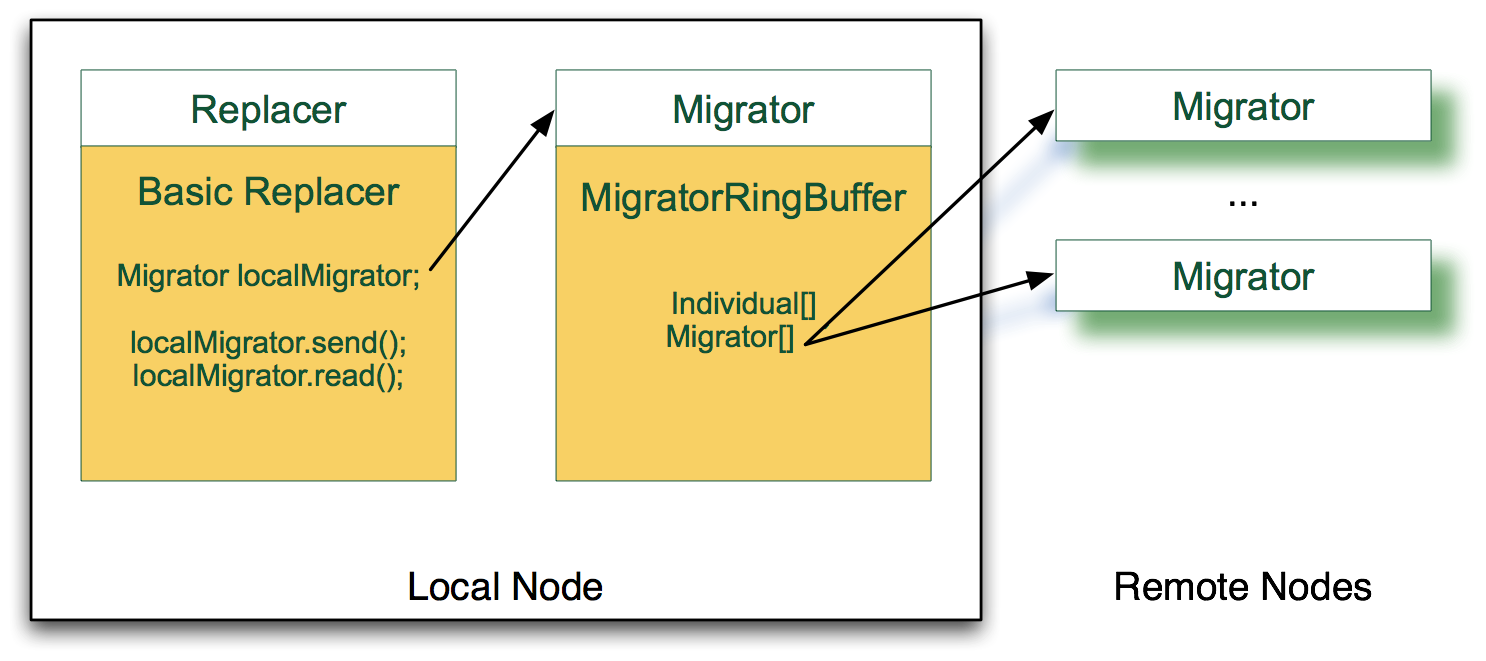
\includegraphics[width=10cm]{gfx/osgiliath/migrator.png}


\caption{Using the Migrator service to create a distributed island EA with a ring topology (white boxes are service interfaces and orange boxes are implementations).}
\label{MIGRATOR}
\end{SCfigure}

% Cada algoritmo debe ser como un paper. No te puedes ir a
% Experimental results para saber qué diablos quieres probar y cómo
% quieres hacerlo. Además, tienes que introducir el resto del capítulo
% y exponer la línea argumental del mismo y como contribuye a la
% tesis. Perdón, LA TESIS - JJ FERGU: teniendo en cuenta todo esto, como estarás viendo

\subsection{Implementation and Deployment}

All services have been implemented in OSGiLiath. The {\em Migrator} and {\em Algorithm} services are exposed using ECF Generic Server, as explained in Section \ref{sec:osgiliath:technology}). This services are, therefore, automatically bound to each node in the clusters, without notify their IP address. Extra code to manage the communication has not been added, as all services are undistinguishable of being remote or local. Remote {\em Migrators} and {\em Algorithms} are bound thanks to the bind/unbind methods of declarative services and ECF (explained in Section \ref{sec:osgiliath:technology}). Several properties can added to the service allows to ECF automatically announce the implementation to all nodes in the network and no specific code is required to change from one distribution mechanism to another.

The services have been deployed in two different computational systems: a {\em
  heterogeneous cluster} % no es un cluster, simplemente un grupillo
                         % de ordenadores - JJ
and a {\em homogeneous cluster}. The first
one is formed by four different computers of our lab with different
processors, operating systems and memory size. The latter is a
dedicated scientific cluster formed by homogeneous nodes. Table
\ref{tabcomputers} shows the features of each system and the name of
the nodes. % El espacio HeHa es muy amplio. Podrías haber probado
           % diferentes configuraciones de este: más diferencia, menos
           % diferencia... de hecho, deberías hacerlo para esta tesis
           % (y trabajos posteriores) - JJ

\begin{SCtable}[][t]
\resizebox{11cm}{!}{
\begin{tabular}{|c|c|c|c|c|}
\hline
\rowcolor{colorCorporativoSuave}Name     & Processor  & Memory  & Operating System  & Network  \\ \hline \hline
\multicolumn{5}{|>{\columncolor{colorCorporativoMasSuave}}c|}{Homogeneous cluster} \\ \hline
\rowcolor{colorCorporativoSuave}HoN[1-4] &  Intel(R) Xeon(R) CPU   E5320  @ 1.86GHz       & 4GB & CentOS 6.7    &   Gigabit Ethernet    \\ \hline
\hline
\multicolumn{5}{|>{\columncolor{colorCorporativoMasSuave}}c|}{Heterogeneous cluster} \\ \hline
\rowcolor{colorCorporativoSuave}HeN1  &  Intel(R) Core(TM)2 Quad CPU    Q6600  @ 2.40GHz    & 4GB   & Ubuntu 11.10 (64 bits)  & Gigabit Ethernet      \\ \hline
\rowcolor{colorCorporativoMasSuave}HeN2  &  Intel(R) Core(TM)2 Quad CPU    Q6600  @ 2.40GHz    & 4GB   & Ubuntu 11.04 (64 bits)  & Gigabit Ethernet      \\ \hline
\rowcolor{colorCorporativoSuave}HeN3  &  AMD Phenom(tm) 9950 Quad-Core Processor @ 1.30Ghz    & 3GB   & Ubuntu 10.10 (32 bits)  & 100MB Ethernet      \\ \hline
\rowcolor{colorCorporativoMasSuave}HeN4  &  Intel (R) Pentium 3 @ 800MHz               & 768 MB  & Ubuntu 10.10 (32 bits)  &   10MB Ethernet     \\ \hline
\end{tabular}
\caption{Details of the clusters used: a homogeneous cluster (Ho), and a heterogeneous cluster (He)}
\label{tabcomputers}
}
\end{SCtable}

\section{Experimental results}

Once the services have been created, the different combinations of systems and parameter are evaluated. Table \ref{table:parameters} summarizes all the parameters used in the
experiments. % ¿Explicación? ¿Has probado otros?  - JJ




                                \begin{SCtable}[][t]{
\begin{tabular}{ccccc} \hline
\rowcolor{colorCorporativoSuave}Node        & HeN1     & HeN2      & HeN3     & HeN4   \\ \hline \hline
\multicolumn{5}{>{\columncolor{colorCorporativoMasSuave}}c}{MMDP problem} \\ \hline
\rowcolor{colorCorporativoSuave}Generations & 10990.25 & 10732.075 &  7721.15 & 717.95 \\ \hline
\rowcolor{colorCorporativoMasSuave}Proportion  & 36.43    & 35.58    & 25.59    & 2.38    \\ \hline
\multicolumn{5}{>{\columncolor{colorCorporativoSuave}}c}{OneMax problem} \\ \hline
\rowcolor{colorCorporativoMasSuave}Generations & 2430.27 & 2353.77 & 1423.77 & 91.5 \\ \hline
\rowcolor{colorCorporativoSuave}Proportion  & 38.58   & 37.36   & 22.6   & 1.45 \\ \hline
\end{tabular}
\caption{Average number of generations in each node needed to find the
  optimum on the heterogeneous cluster with heterogeneous size.}
\label{table:generations}
}
\end{SCtable}











\begin{SCtable}[][t]
\resizebox{11cm}{!}{
\begin{tabular}{cc}
\hline
\rowcolor{colorCorporativoSuave}Name & Value\\ \hline \hline
\rowcolor{colorCorporativoMasSuave}Crossover type & Two-point crossover \\ \hline
\rowcolor{colorCorporativoSuave}Crossover rate & 0.5\\ \hline % muy
                                % bajo probablemente.
\rowcolor{colorCorporativoMasSuave}Mutation probability of each gene & 1/individual size\\
\hline % esa no es una tasa de mutación, es determinista. ¿Todos
       % mutan? - JJ FERGU: arreglado
\rowcolor{colorCorporativoSuave}Selection & 2-tournament \\ \hline
\rowcolor{colorCorporativoMasSuave}Replacement & Steady-state\\ \hline
\rowcolor{colorCorporativoSuave}Generations to migrate & 64 \\ \hline
\rowcolor{colorCorporativoMasSuave}Number of individuals to migrate & 1 \\ \hline
\rowcolor{colorCorporativoSuave}Stop criterion & Optimum found \\ \hline
\rowcolor{colorCorporativoMasSuave}Individual size for MMDP & 150 \\ \hline
\rowcolor{colorCorporativoSuave}Individual size for OneMax & 5000 \\ \hline
\rowcolor{colorCorporativoMasSuave}Runs per configuration & 40 \\ \hline
\hline
\rowcolor{colorCorporativoSuave}Total individuals in HoSi and HeSi & 1024\\ \hline \hline
\rowcolor{colorCorporativoMasSuave}Sub-population size in each node in HoSi & 256  \\ \hline
\rowcolor{colorCorporativoSuave}Sub-population sizes in HeSi for MMDP
& 374, 364, 262 and 24 (from N1 to N4) (see Section \ref{subsec:adaptive:hesisizes})\\ \hline % ¿REsultado? ¿Cómo se
                                % ha obtenido? - JJ FERGU: añado referencia
\rowcolor{colorCorporativoMasSuave}Sub-population sizes in HeSi for OneMax & 396,  382, 232 and 14 (from N1 to N4) (see Section \ref{subsec:adaptive:hesisizes})\\ \hline
\hline
\rowcolor{colorCorporativoSuave}Maximum island size in AdSi & 1024 \\ \hline
\rowcolor{colorCorporativoMasSuave}Minimum island size in AdSi & 16 \\ \hline
\rowcolor{colorCorporativoSuave}Initial island size in AdSi & 256 \\ \hline 
\end{tabular}
}
\caption{Parameters used in all configurations.}
\label{table:parameters}
\end{SCtable}

%\section{Implementation in OSGiLiath}
%In order to deal with the operating system and architecture
%heterogeneity (different operating systems, processors, compilers,
%etc.), the OSGiLiath framework \cite{SOASOCO}, based in Java, has
%been used in this work. This is a service-oriented evolutionary
%framework that automatically configures the services to be used in a
%local network. In this case, each node offers a migration buffer to
%accept foreign individuals. Also, in order to reduce bottlenecks in
%distributed executions, asynchronous communication has been provided
%to avoid idle time using reception buffers (that is, the algorithm
%does not wait until new individuals arrive, but the buffers cannot be
%used again until the reception is done). This kind of communication
%offers an excellent performance when working with different nodes and
%operating systems, as demonstrated in
%\cite{HETEROGENEOUSHARD,AsynchronousMerelo08}. The transmission
%mechanism is based on ECF Generic server (over
%TCP)\footnote{\url{http://www.eclipse.org/ecf/}}.  The source code of
%the algorithms used in this work is available in
%\url{http://www.osgiliath.org} under a LGPL V3 License. 

% Hombre, para una cosa que nombra Osgiliath, lo quitas - JJ FERGU: añadido arriba, es que revisaste esto mu pronto! xD

The three main objectives of parallel programming are to tackle large
computational problems, increase the performance of algorithms in a
finite time, or reduce computational time to solve the problem
(reaching the optimum). In this chapter, we focus in the last
objective. % Y a los otros dos, que les den - JJ
As claimed by \person{Alba and Luque} in
\cite{Alba06evaluationParallel}, assessing the performance of a
parallel EA by the number of fitness function evaluations required to
attain a solution may be misleading. In our case, for example, the
evaluation time is different in each node of the heterogeneous
cluster, so the real algorithm speed could not be reflected
correctly. %¿Cuál es la velocidad "real"? - JJ
 However, the number of evaluations has been included in
this chapter to better understanding the results. % ¿Better que qué? - JJ
The total number of
generations carried out by all nodes, and the maximum number of
generations required by the faster node in each configuration are also
shown. It is difficult to compare the performance of HoHa and HeHa for
the same reason: the evaluation time is different in each system (and
even in each node). Thus, one of the objectives in this chapter is not
making the heterogeneous cluster comparable or better in time than the
homogeneous one (because they are, obviously, different), but showing
that the same parameter configuration can improve performance in time
on heterogeneous clusters and could not have an effect on homogeneous
ones. 
% es que, al final, estás comparando cosas que no son comparables. Si
% el cluster homogéneo es más rápido, tendrá mejores
% resultados. Tendrías que haber hecho un montaje experimental un poco
% mejor: sustituir un ordenador del cluster por uno más potente, por
% uno menos potente, dos del cluster por esos dos, luego tres, y lo
% que sea. Como parte de la tesis, deberías diseñar una metodología
% para hacer este tipo de experimentos - JJ FERGU: es que no comparo clusters entre sí, mira los boxplots como están separados. El homogéneo lo uso para ver si la mejora se debe al conjunto de parámetros o a la combinación de parámetros y hardware.

\subsection{Obtaining the HeSi sizes}
\label{subsec:adaptive:hesisizes}
After executing the algorithm 40 times per problem on the
heterogeneous cluster, % ¿Por qué? - JJ
we have obtained the average number of generations in each node, as it
can be seen in Table \ref{table:generations}. Note how the generations
attained (and their proportion in every node) to reach the optimum
depends on the problem considered (besides the hardware). % Jolines,
                                % cómo no va a depender en el problema
                                % - JJ

\subsection{MMDP results}

Table \ref{tab:resultsMMDP} shows the results for the MMDP
problem. These results are also shown in the boxplots of Figure
\ref{fig:timeMMDP} (time) and Figure \ref{fig:evalsMMDP}
(evaluations). Table \ref{tab:significanceMMDP} shows the statistical
significance of the results. First, a Kolmogorov-Smirnov test is
performed to assess the normality of the distributions. As all
distributions are not normal, we use non-parametric tests. To compare
between two methods (HoSi and HeSi in the homogeneous cluster) a
Wilcoxon test has been applied. For a three methods comparison (HoSi,
HeSi and AdSi on heterogeneous cluster) a Kruskal-Wallis test has been
used. % y esto lo haces porque... ¿Debe todo el mundo saber esto? -JJ

 In the HeHa system,  offline adaptation of  the sub-population to the computational
 power of each node makes the algorithm finish significantly earlier,
 and also, needing a lower number of evaluations to reach the solution. On the other hand, in the HoHa system,
 setting the same sub-population sizes makes no difference in time and
 evaluations, that is, changing this parameter has no influence in the
 algorithm's performance (p-value=0.52 for time and 0.08 for
 evaluations). % esto es interesante porque... - JJ


\begin{SCtable}[][t]
\resizebox{11cm}{!}{
\begin{tabular}{ccccc}
\hline
\rowcolor{colorCorporativoSuave}Configuration & Max. generations      & Total generations     &   Total evaluations     & Time (ms) \\ \hline \hline
\rowcolor{colorCorporativoMasSuave}HoSi/HeHa & 11194.8 $\pm$ 18810.08   & 30161.42 $\pm$  50722.03 & 7723372.8 $\pm$  12984841.71   & 27871.075 $\pm$  44583.14 \\ \hline
\rowcolor{colorCorporativoSuave}HeSi/HeHa   & 2506.1  $\pm$5308.872    & 8683.9    $\pm$ 18459.58 &  2453677 $\pm$5217896.18  &  8110.9 $\pm$ 17162.86 \\ \hline
\rowcolor{colorCorporativoMasSuave}AdSi/HeHa   & 2407.10 $\pm$3938.43     & 8376.35 $\pm$ 14140.55   & 2948946.15  $\pm$  5165324.99 &  10235.89  $\pm$ 17193.98\\ \hline  \hline
\rowcolor{colorCorporativoSuave}HoSi/HoHa   & 2614    $\pm$5889.93     & 10259.22  $\pm$ 23153.23 &  2628409.6 $\pm$   5927278.22 & 11560.8 $\pm$ 26072.14 \\ \hline
\rowcolor{colorCorporativoMasSuave}HeSi/HoHa   & 5411.92 $\pm$15608.81    & 10689.15  $\pm$  30790.7 & 1844908.1 $\pm$  5314771.88 &  9520.325 $\pm$   27237.35 \\ \hline

\end{tabular}
}
\caption{Results for the MMDP problem}
\label{tab:resultsMMDP}
\end{SCtable}




\begin{SCfigure}[tb]
\centering

%\subfigure[Heterogeneous cluster]{
   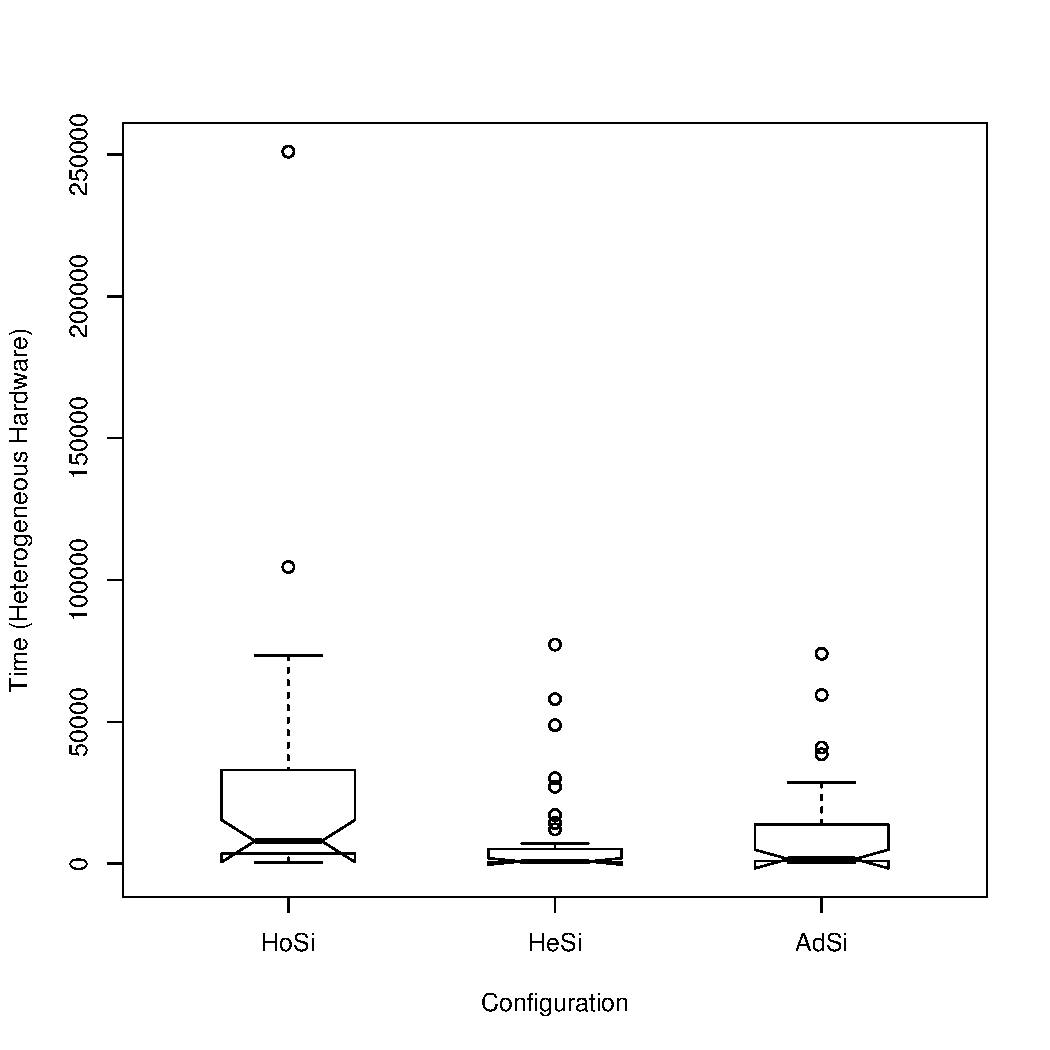
\includegraphics[scale =0.4] {gfx/adaptiveresults/timeMMDPhetero.pdf}
   \label{fig:subfig1}
%}
%\subfigure[Homogeneous cluster]{
   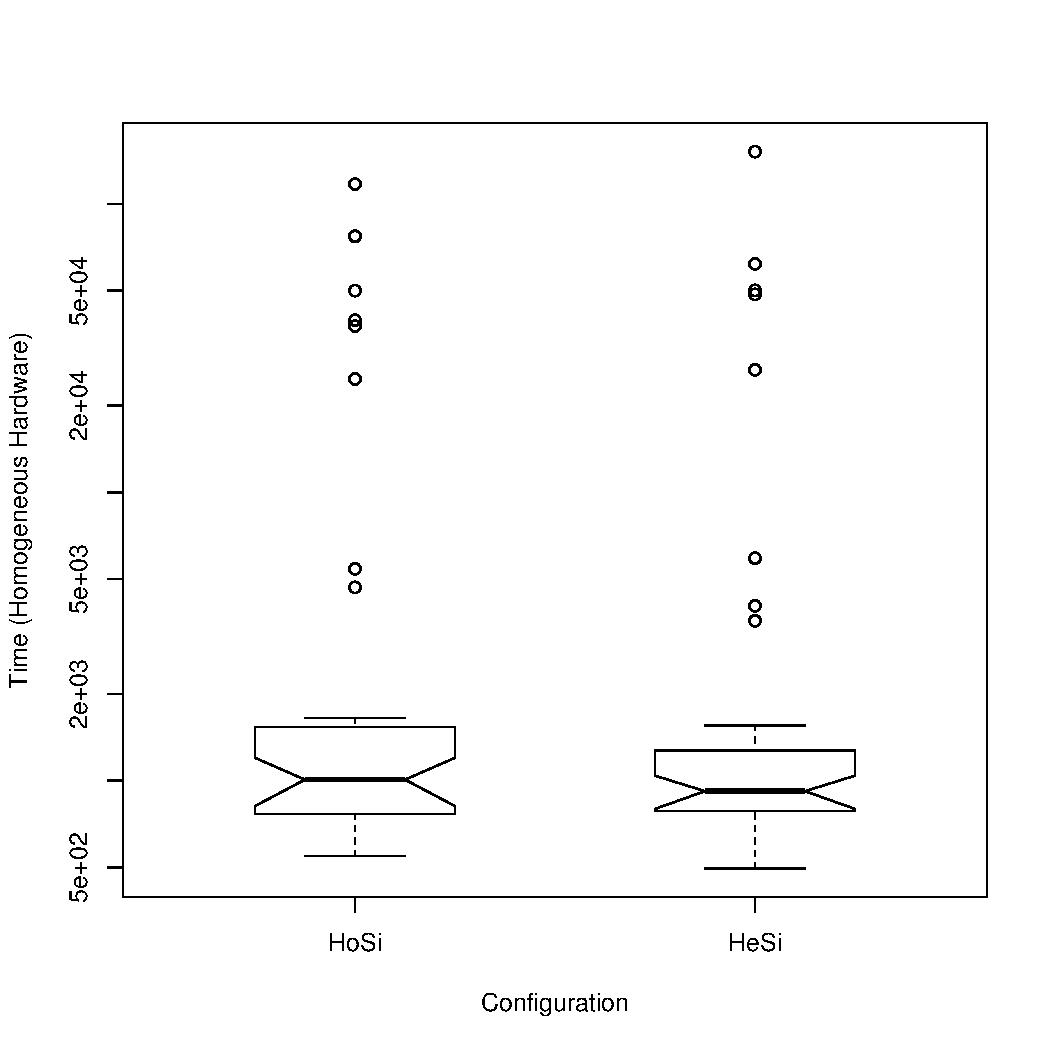
\includegraphics[scale =0.4] {gfx/adaptiveresults/timeMMDPhomo.pdf}
   \label{fig:subfig2}
% }
\caption{Time to obtain the optimum in the MMDP problem
  (milliseconds).}

\label{fig:timeMMDP}
\end{SCfigure}

\begin{SCfigure}[tb]
\centering

%\subfigure[Heterogeneous cluster]{
   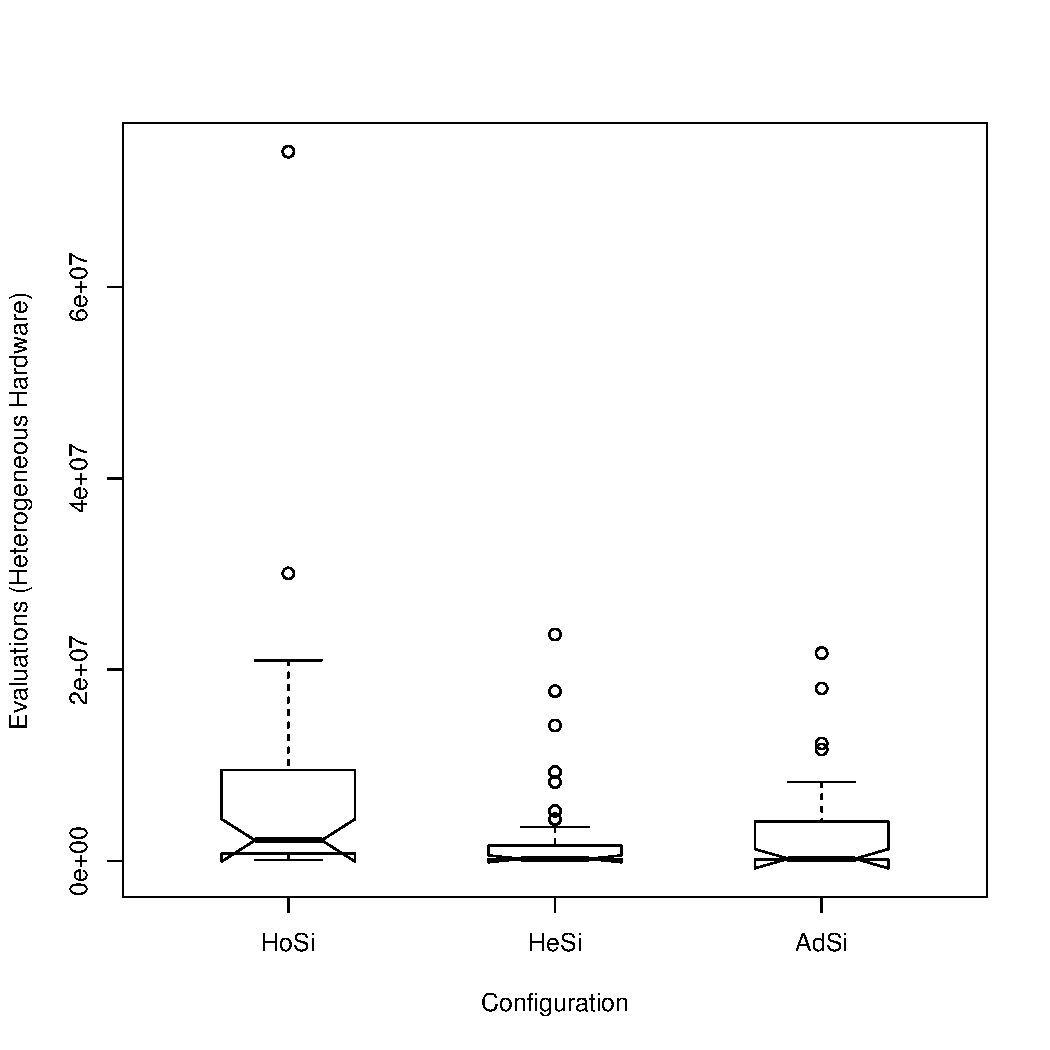
\includegraphics[scale =0.4] {gfx/adaptiveresults/evalsMMDPhetero.pdf}
   \label{fig:subfig1}
 %}
%\subfigure[Homogeneous cluster]{
   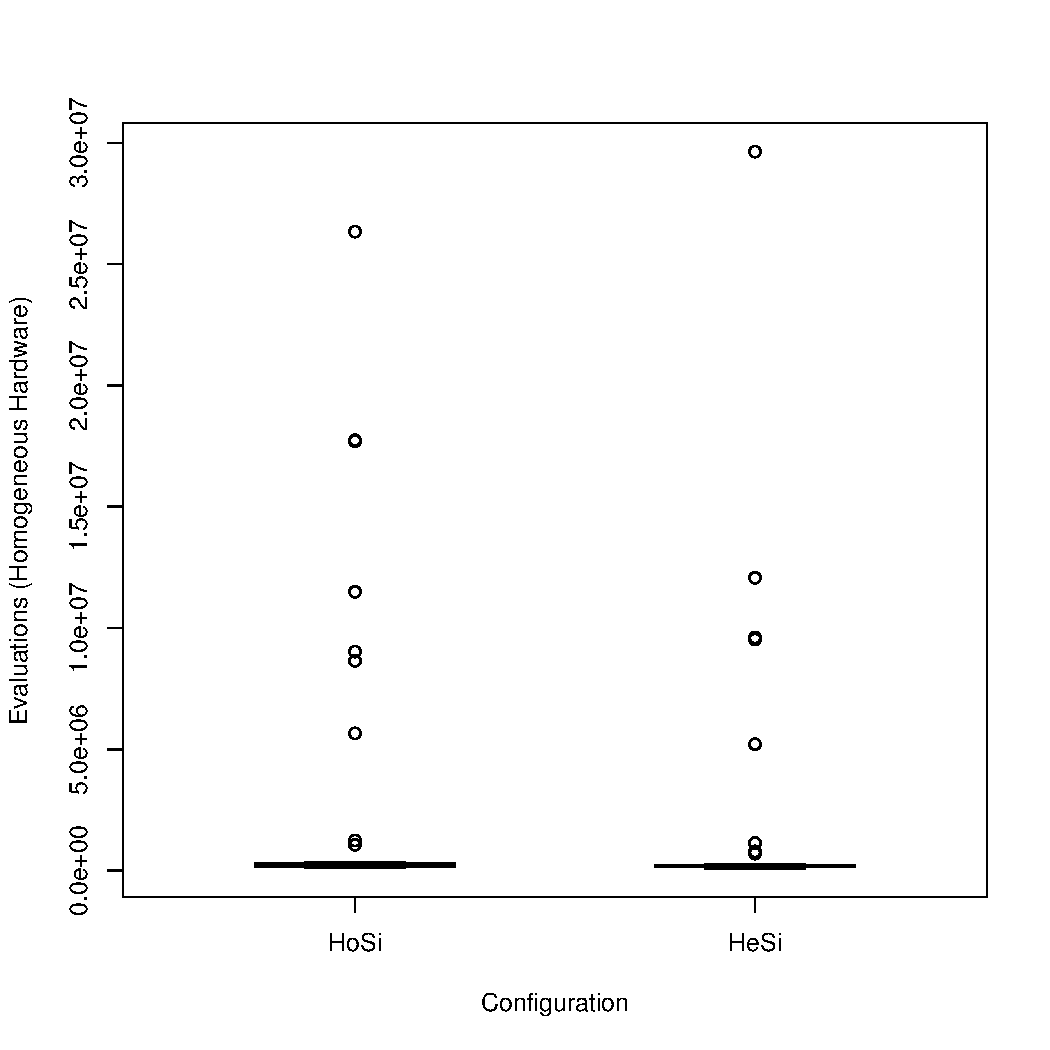
\includegraphics[scale =0.4] {gfx/adaptiveresults/evalsMMDPhomo.pdf}
   \label{fig:subfig2}
 %}
\caption{Number of evaluations for MMDP problem.}
\label{fig:evalsMMDP}
\end{SCfigure}



To see the differences on how the evolution is being performed, the
average fitness in each node of HeHa is shown in Figures
\ref{fig:hosiheha} and \ref{fig:hesiheha}. As it can be seen, with the
HeSi (Figure \ref{fig:hesiheha}), the local optima are overtaken in
less time than HoSi (Figure \ref{fig:hosiheha}).  This can be
explained because in HeSi, the migration from HeN4 to HeN1 is
performed faster, adding more heterogeneity to the whole system. Gaps
in the figures correspond to the time spent in the nodes for sending
the migrant individual to other nodes (not while they are receiving
them). %no se entiende - JJ
 In the HoHa configurations, the evolution of sub-population is
 performed at the same time, being the average fitness similar for all
 nodes during all runs.  


\begin{SCfigure}[tb]
\centering
 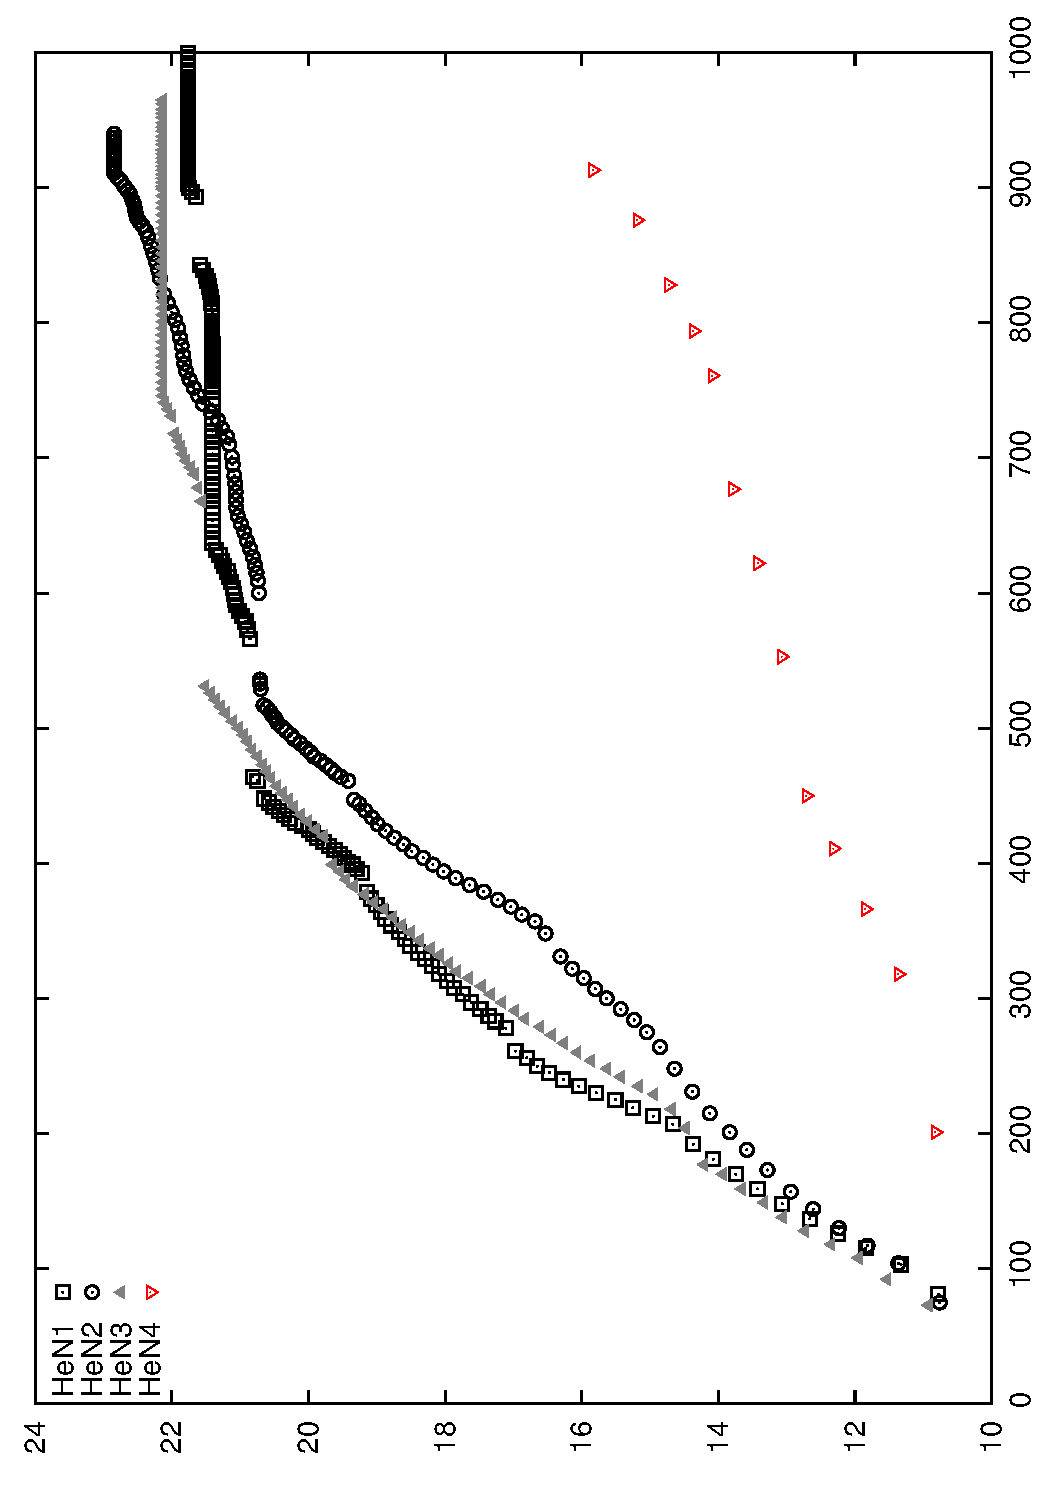
\includegraphics[angle=-90,scale =0.4] {gfx/adaptiveresults/generationsMMDPhomosize.pdf}
\caption{Average fitness in the first 1000 milliseconds of execution of the four nodes of the heterogeneous cluster with the same sub-population sizes (HoSi/HeHa) for the MMDP problem.}
\label{fig:hosiheha}
\end{SCfigure}

\begin{SCfigure}[tb]
\centering
 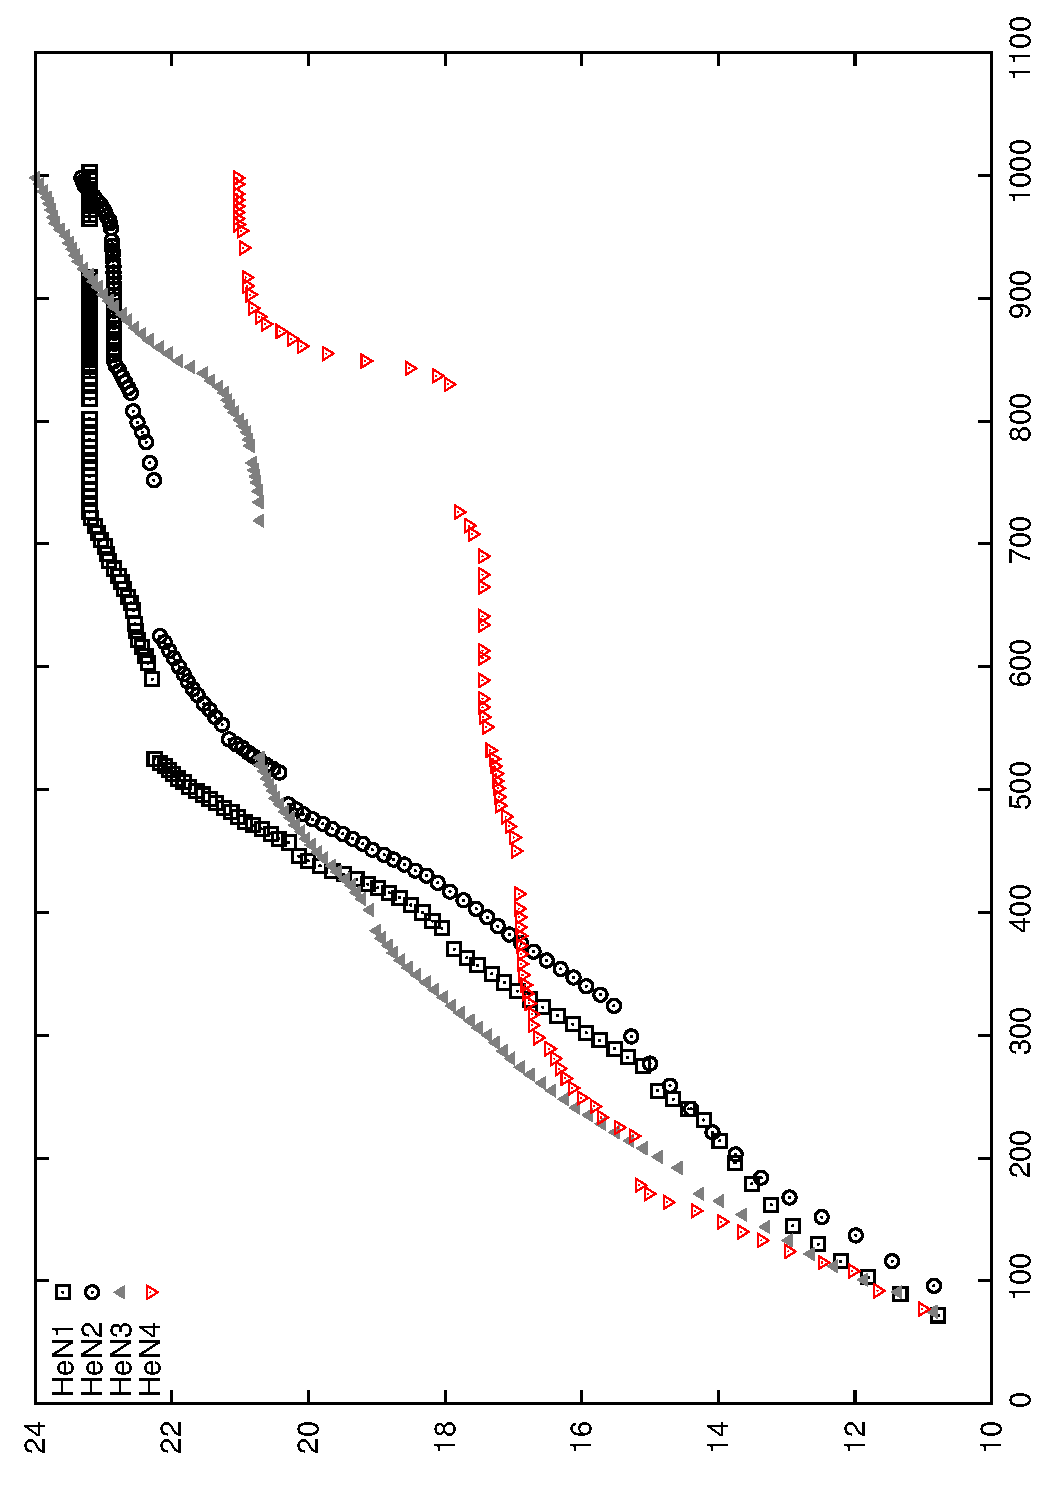
\includegraphics[angle=-90,scale =0.4] {gfx/adaptiveresults/generationsMMDPheterosize.pdf}
\caption{Average fitness in the first 1000 milliseconds of execution of the four nodes of the heterogeneous cluster with different sub-population sizes (HeSi/HeHa) for the MMDP problem.}
\label{fig:hesiheha}
\end{SCfigure}

With respect to AdSi/HeHa, %agh, regarding to. ¡Amoragismos no! - JJ FERGU: a lo mejor lo puso él xD (lo cambio).
results are significantly  equal (p-value 0.139) to HeSi/HeHa (and, therefore, better than HoSi/HeHa), but this time no previous tuning has been required.  Average sub-population sizes in each node are shown in Table \ref{table:sizesMMDP}. The proportions of size are similar to the proportions in Table \ref{table:generations}. Figure \ref{fig:sizesMMDP} plots all the possible sizes in each node during all the runs. This figure shows that the variation of the sub-population sizes lies proportionally to the computational power of each node. The outliers in boxplots are produced during the size changing, as it can be seen in Figure \ref{fig:sizesMMDP1ejec}. As N4 is the slower node with difference it keeps its size always close to the minimum (16 individuals).

\begin{SCfigure}[tb]
\centering
 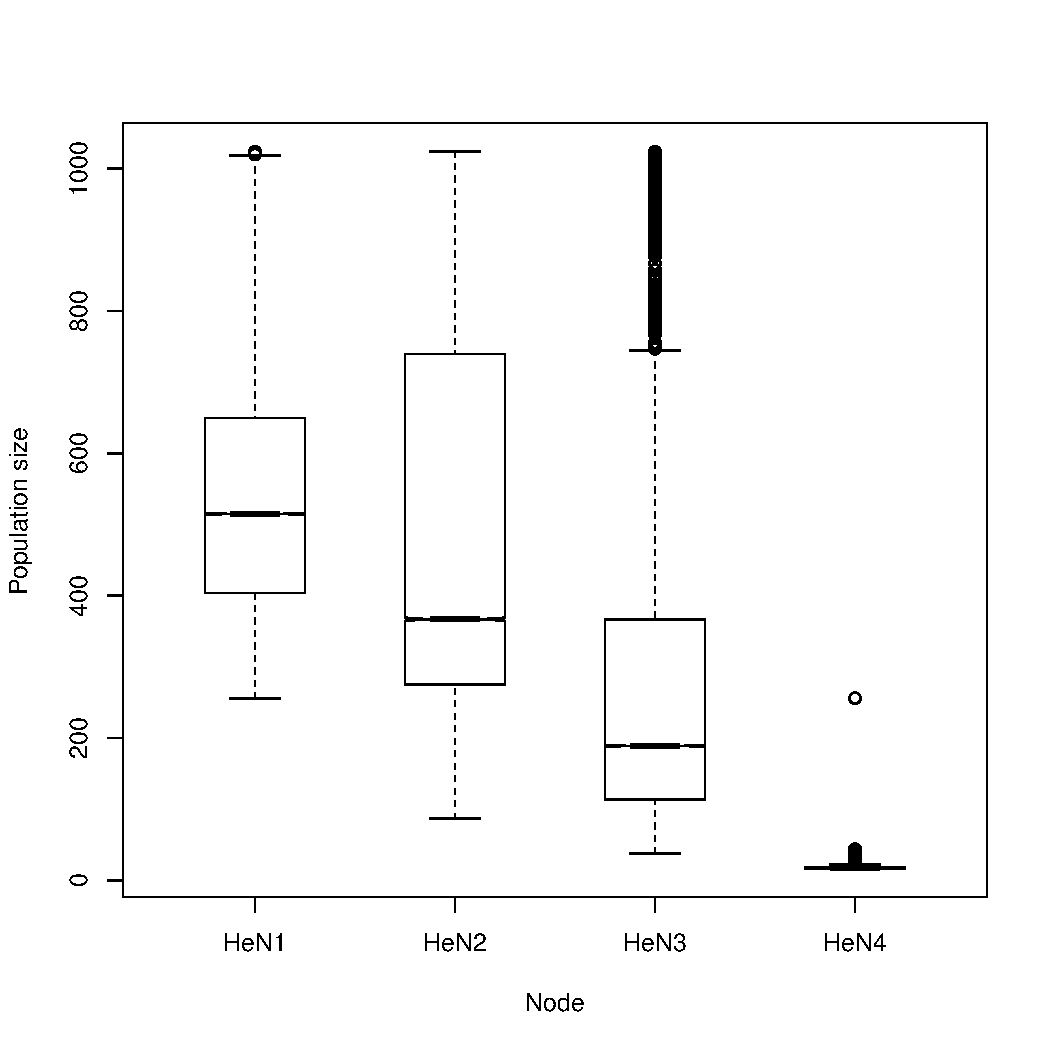
\includegraphics[scale =0.4] {gfx/adaptiveresults/sizesMMDP.pdf}
\caption{Boxplots of the sub-population sizes in each node during all the runs for the MMDP problem.}
\label{fig:sizesMMDP}
\end{SCfigure}

\begin{SCfigure}[tb]
\centering
 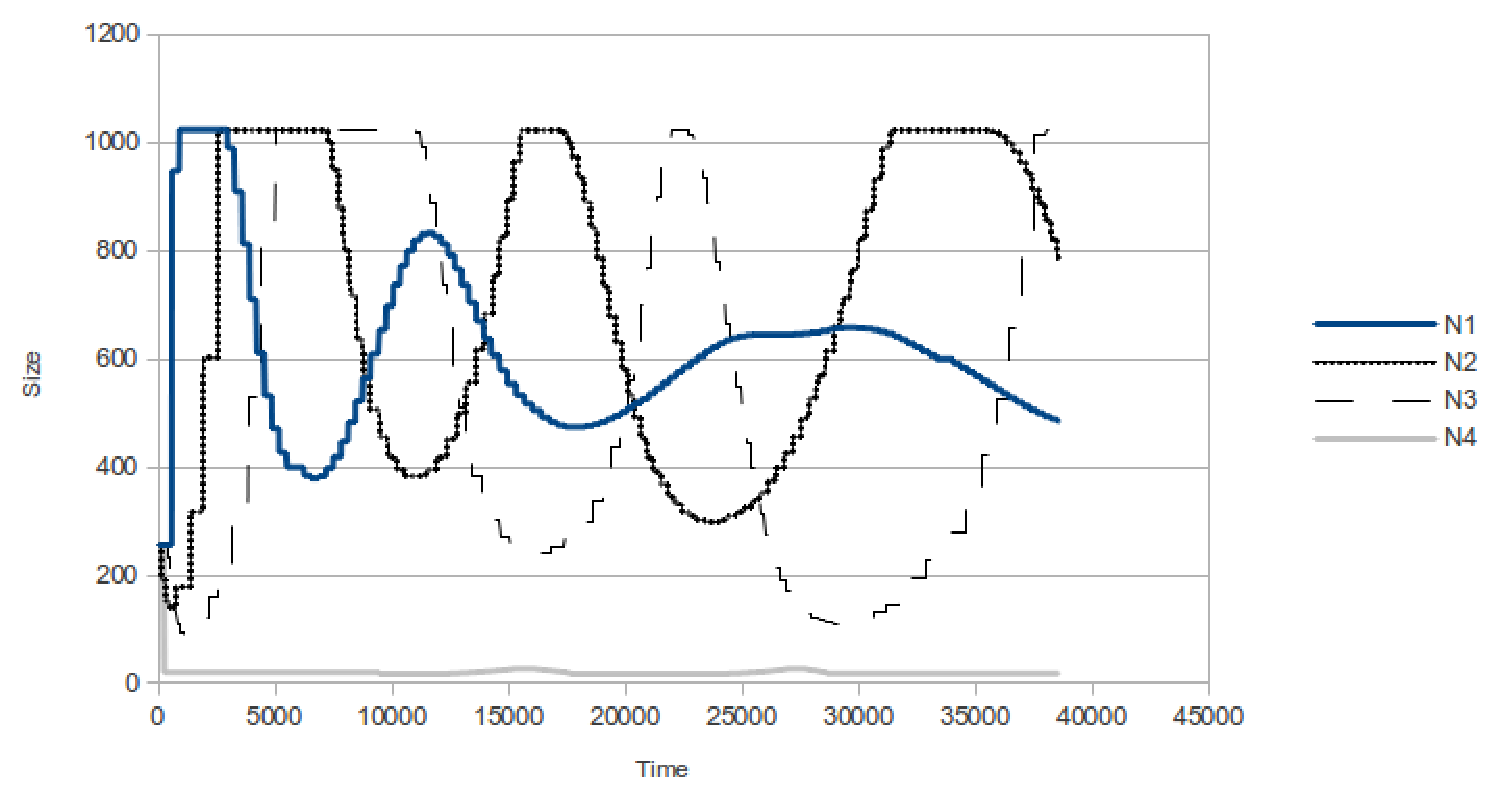
\includegraphics[scale =0.4] {gfx/adaptiveresults/sizesMMDP1ejec.pdf}
\caption{Population size in each node during one execution to solve the MMDP problem.}
\label{fig:sizesMMDP1ejec}
\end{SCfigure}



\begin{SCtable}[][tb]
\resizebox{6cm}{!}{
\begin{tabular}{ccccc}
\hline
\rowcolor{colorCorporativoSuave}Node        & HeN1     & HeN2      & HeN3     & HeN4   \\ \hline \hline
\rowcolor{colorCorporativoMasSuave}Size &  556.31 & 504.30  & 321.15 & 19.81 \\ \hline
\rowcolor{colorCorporativoSuave}Proportion  & 39.69 &  35.98 & 22.91 & 1.41   \\ \hline
\end{tabular}
\caption{Average sub-population size in each node on the heterogeneous cluster with adaptive size (MMDP).}
\label{table:sizesMMDP}
}
\end{SCtable}



Summarizing, adapting the sub-population sizes to the computational
power of each machine (offline and online) has reduced the time to
obtain the optimum. The same heterogeneous fixed sizes in the
homogeneous cluster does not produce a significant decrease of running
time, so the improvement is produced by the heterogeneity and not due
to the different island sizes. Moreover, the AdSi proposal is not
applicable in HoHa because there are not differences of generations
during runtime. % y esto es interesante porque... - JJ

\subsection{OneMax results}

Results for this problem are shown in Table \ref{tab:onemaxresults} and Figures  \ref{fig:timeOneMax} and \ref{fig:evalsOneMax}. In this case, adapting offline the sub-population sizes significantly decreases  the running time for solving it in the heterogeneous cluster, but this time, the number of evaluations is increased (see statistical significance in Table \ref{tab:significanceONEMAX}). In the homogeneous system, the effect of changing the sub-population sizes is clearer, and this time the number of evaluations (and therefore, the time) are reduced (both significantly). 

The efficiency to resolve OneMax problem depends mainly on the ability to mix
% ¿onemax es el que es eficiente? ¿resolverlo lo es? - JJ FERGU: arreglado
the building-blocks, and less on the genetic diversity and size of the
population (as with MMDP). No genetic diversity is particularly
required. When properly tuned, a simple Genetic Algorithm is able to
solve OneMax in linear time. Sometimes, problems like OneMax are used
as control functions, in order to check if very efficient algorithms
on hard functions fail on easier ones. As it can be seen in Figure
\ref{fig:gensonemaxhomosize}, the average fitness of all sub-populations
are increasing in linear way in the HoSi/HeHa configuration. However,
the slower node evaluates extremely fewer times.  On the other
side, in Figure \ref{fig:gensonemaxheterosize}, smaller sub-population
sizes make that slower nodes increase the number of evaluations, % make that? increase the? Los nodos lo hacen? ¡Gramática! - JJ
but the average fitness is also maintained in linear way (and in
smaller increase rate) between migrations. Nevertheless, the other
nodes still perform a higher number of evaluations. That is the
reason why the number of evaluations is higher in HeHa, and lower in
HoHa. Computational time is more efficiently spent in faster nodes,
having a higher chance to cross the individuals. %¿so es consecuencia
                                %o causa de lo primero? - JJ
 In addition, due to
the larger size of  individuals in the OneMax problem (5000 bits
vs. 150 of the MMDP), the transmission time is larger, (white gaps in the
figures). % ¿hite gaps qué? - JJ
It also implies that HeN4 sends its best individual to
HeN1 in an extremely large amount of time when using HoSi (every 64
generations). 


\begin{SCtable}[][tb]
\resizebox{11cm}{!}{
\begin{tabular}{ccccc}
\hline
\rowcolor{colorCorporativoSuave}Configuration & Max. generations      & Total generations     &   Total evaluations     & Time (ms) \\ \hline \hline
\rowcolor{colorCorporativoMasSuave}HoSi/HeHa   & 2430.34 $\pm$ 70.16  & 6299.31 $\pm$ 250.87 & 1614673.45  $\pm$  64223.09  &  160713.65 $\pm$   8873.46 \\ \hline
\rowcolor{colorCorporativoSuave}HeSi/HeHa   & 2643.34 $\pm$150.82  & 7969.58 $\pm$214.92 & 1802321.65  $\pm$  30511.96  &  151822.75  $\pm$4764.95 \\ \hline 
\rowcolor{colorCorporativoMasSuave}AdSi/HeHa   & 3698.30 $\pm$ 494.56 & 9465.25 $\pm$ 635.07 & 1149277.43  $\pm$ 58887.13 &  103919.33  $\pm$ 6296.39 \\ \hline \hline
\rowcolor{colorCorporativoSuave}HoSi/HoHa   & 1791.32 $\pm$   31.64& 7111.05 $\pm$125.11 & 1822476.8   $\pm$32029.78  &  141176.1    $\pm$2493.72\\ \hline
\rowcolor{colorCorporativoMasSuave}HeSi/HoHa   & 13698.12 $\pm$ 406.85 & 16012.625 $\pm$  482.61 & 895698.2 $\pm$   29520.99  &  77898.85  $\pm$  2935.57 \\ \hline
\end{tabular}
}
\caption{Results for the OneMax problem.}
\label{tab:onemaxresults}
\end{SCtable}



\begin{SCfigure}[tb]
\centering

%\subfigure[Heterogeneous cluster]{
    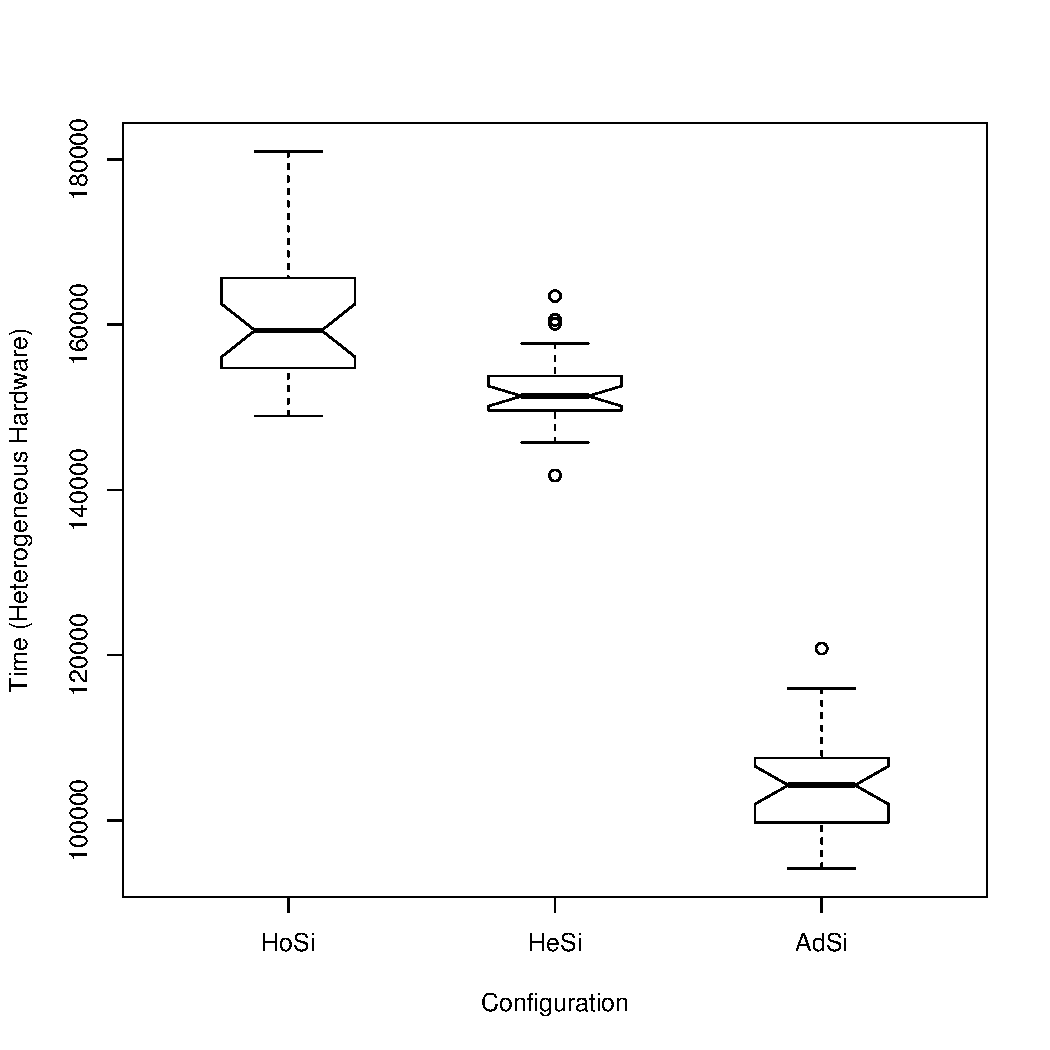
\includegraphics[scale =0.4] {gfx/adaptiveresults/timeONEMAXhetero.pdf}
   \label{fig:subfig1}
 %}
%\subfigure[Homogeneous cluster]{
    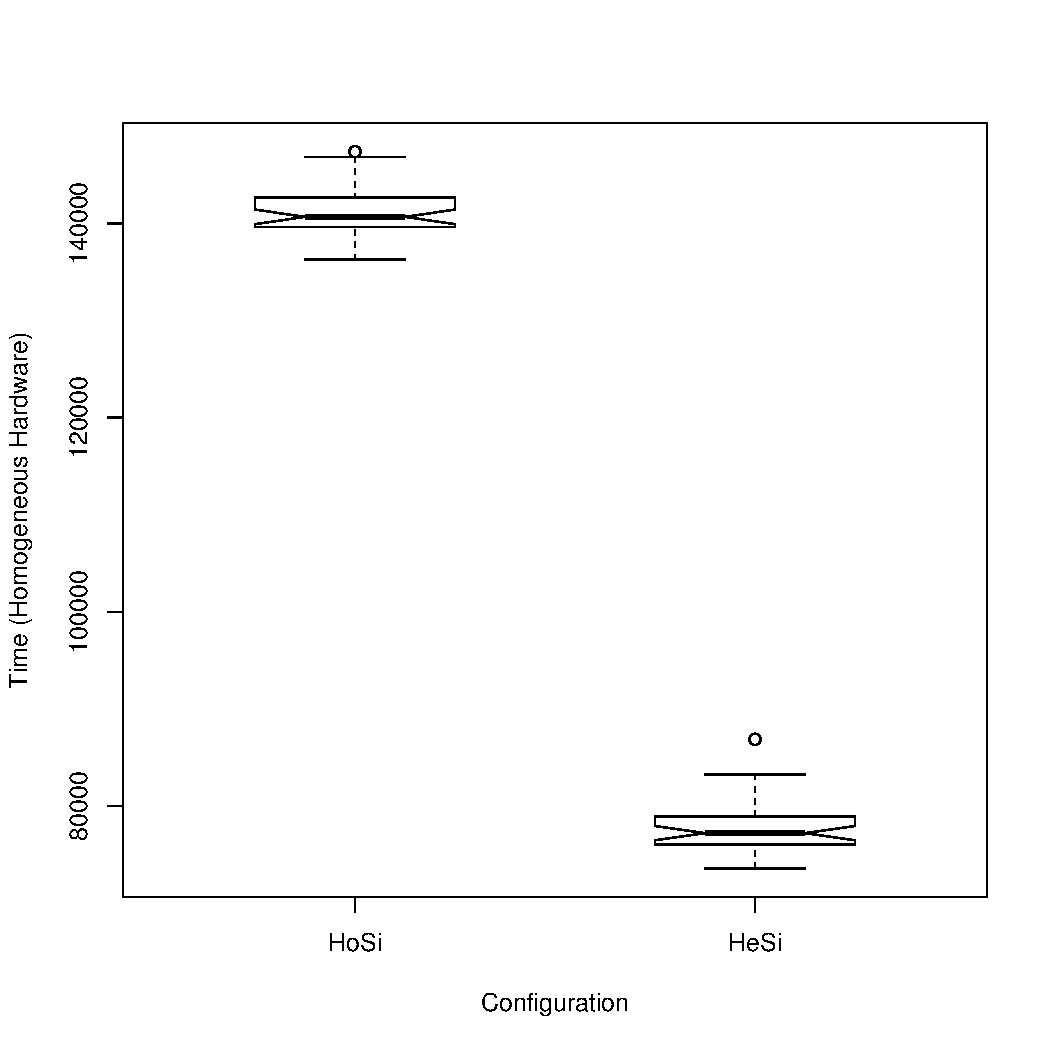
\includegraphics[scale =0.4] {gfx/adaptiveresults/timeONEMAXhomo.pdf}
   \label{fig:subfig2}
 %}
\caption{Time to obtain the optimum in the OneMax problem (milliseconds).}
\label{fig:timeOneMax}
\end{SCfigure}

\begin{SCfigure}[tb]
\centering

%\subfigure[Heterogeneous cluster]{
   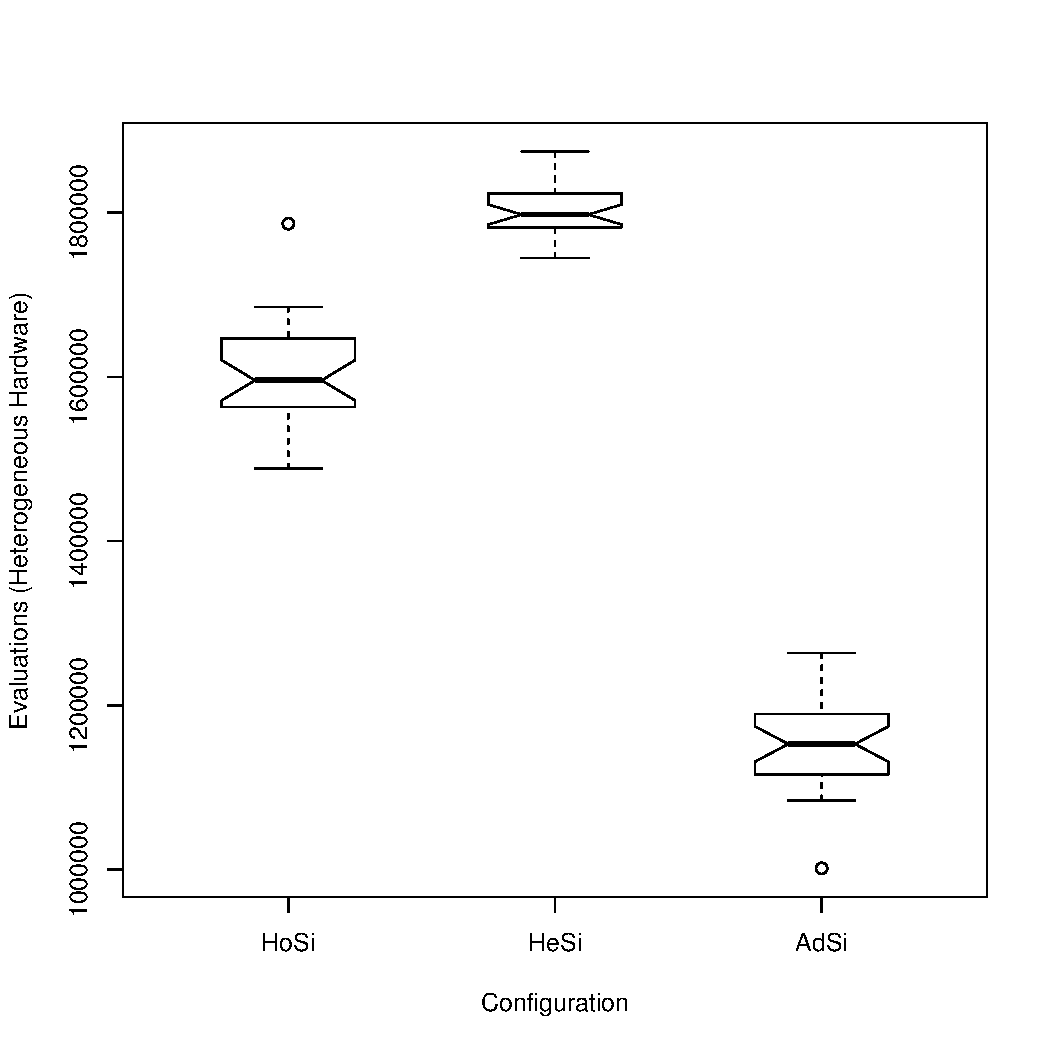
\includegraphics[scale =0.4] {gfx/adaptiveresults/evalsONEMAXhetero.pdf}
   \label{fig:subfig1}
 %}
%\subfigure[Homogeneous cluster]{
   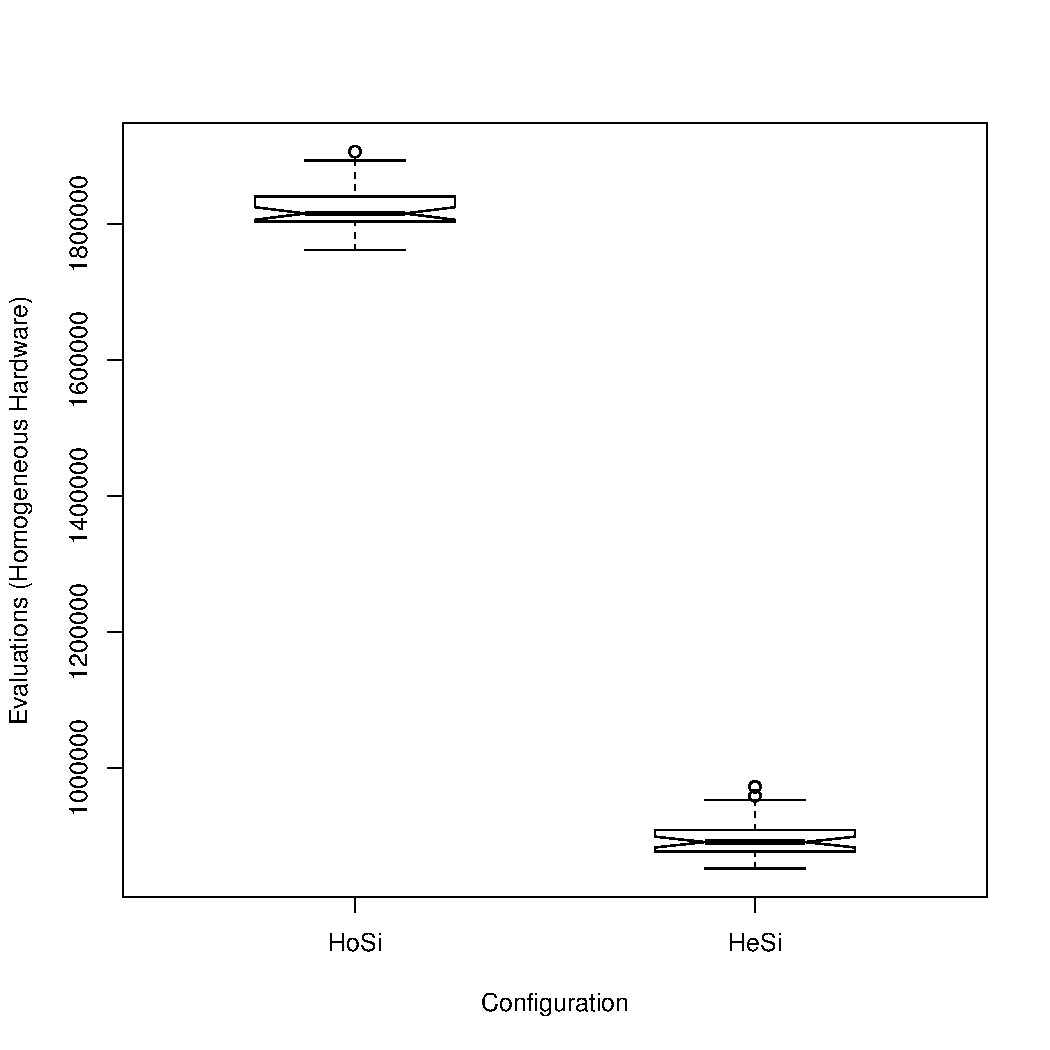
\includegraphics[scale =0.4] {gfx/adaptiveresults/evalsONEMAXhomo.pdf}
   \label{fig:subfig2}
 %}
\caption{Number of evaluations for OneMax problem.}
\label{fig:evalsOneMax}
\end{SCfigure}



\begin{SCfigure}[tb]
\centering 
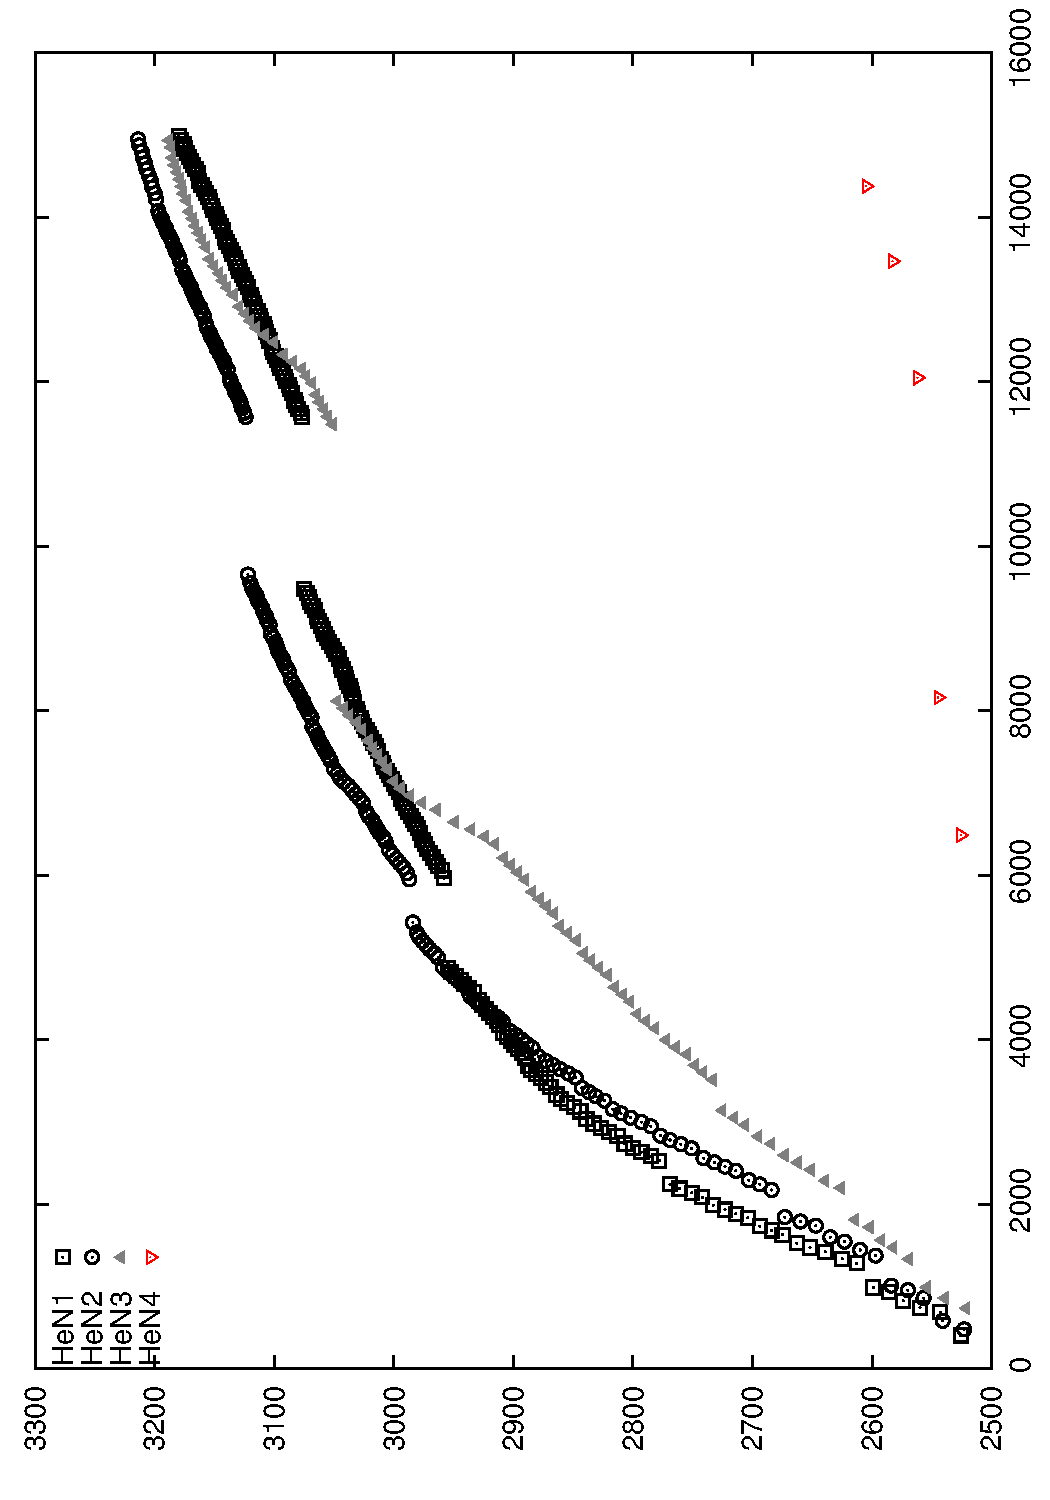
\includegraphics[angle=-90,scale =0.4] {gfx/adaptiveresults/generationsONEMAXhomosize.pdf}
\caption{Average fitness in the first 15000 milliseconds of execution of the four nodes of the heterogeneous cluster with the same sub-population sizes (HoSi/HeHa) for the OneMax problem.}
\label{fig:gensonemaxhomosize}
\end{SCfigure}

\begin{SCfigure}[tb]
\centering
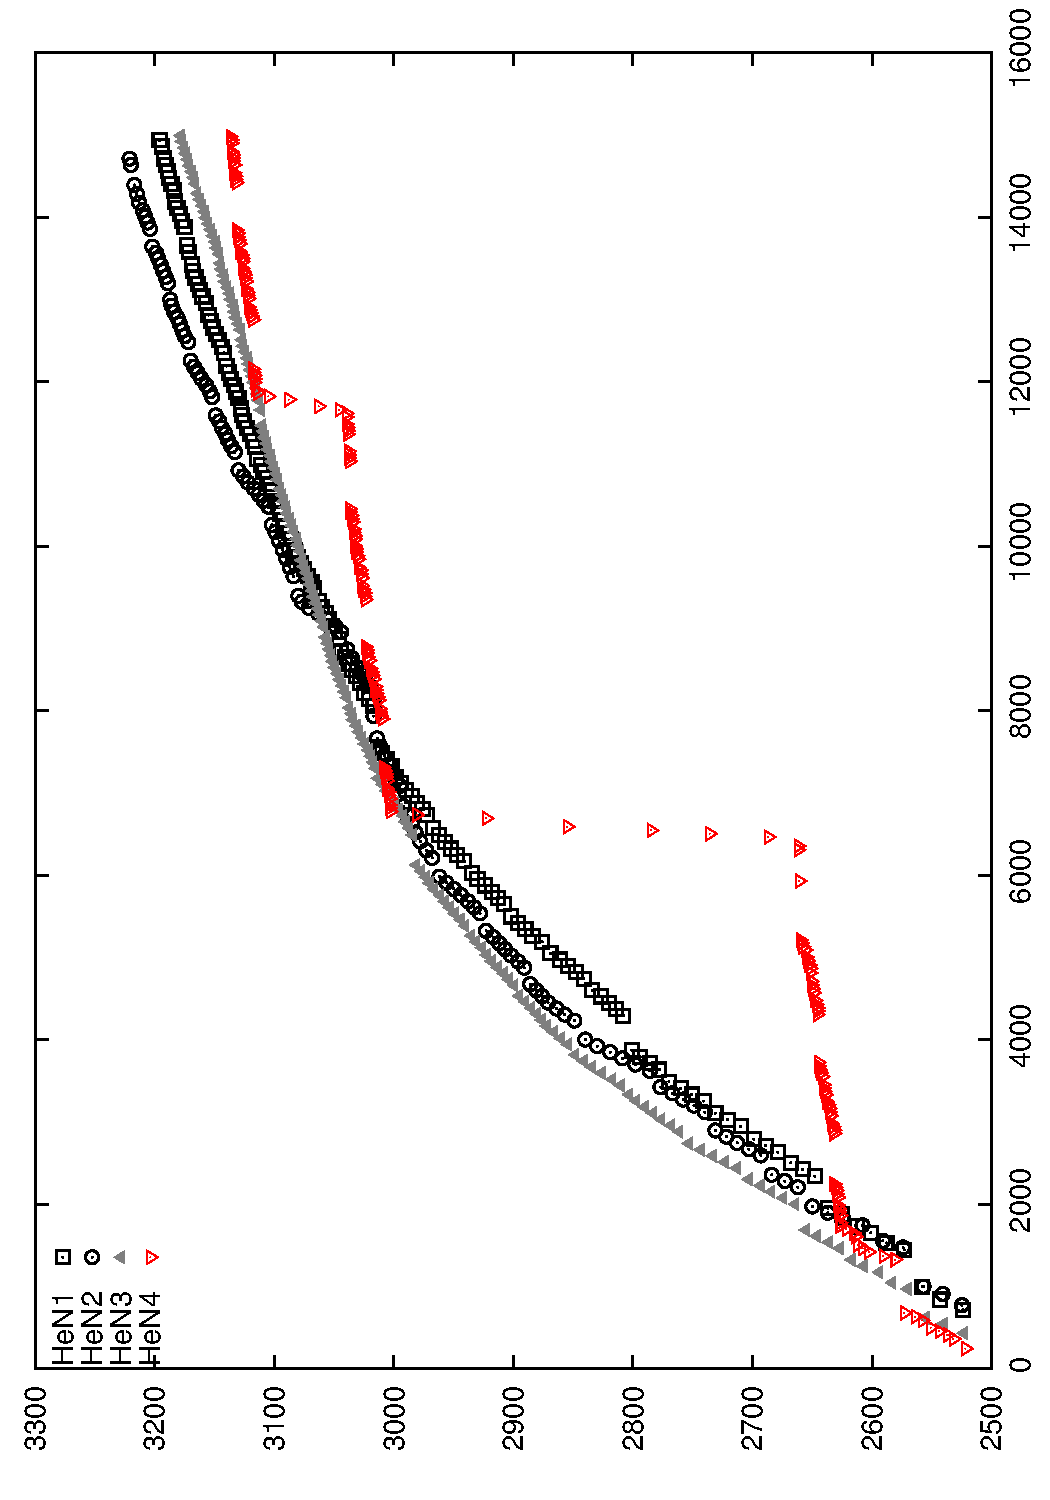
\includegraphics[angle=-90,scale =0.4] {gfx/adaptiveresults/generationsONEMAXheterosize.pdf}
\caption{Average fitness in the first 15000 milliseconds of execution of the four nodes of the heterogeneous cluster with different sub-population sizes (HeSi/HeHa) for the OneMax problem.}
\label{fig:gensonemaxheterosize}
\end{SCfigure}


In the AdSi/HeHa configuration significantly better results in terms of execution time (and number of evaluations) are also attained, and even better than those obtained with HeSi. Average sizes (Table \ref{table:sizesONEMAX}) and boxplots (in Figure \ref{fig:sizesONEMAX}) during all the runs also show proportionality to the computational power of each machine. As in MMDP case, some oscillations (outliers in boxplots) may appear during the execution (as it can be seen in Figure \ref{fig:sizesONEMAX1ejec}).

\begin{SCfigure}[tb]
\centering
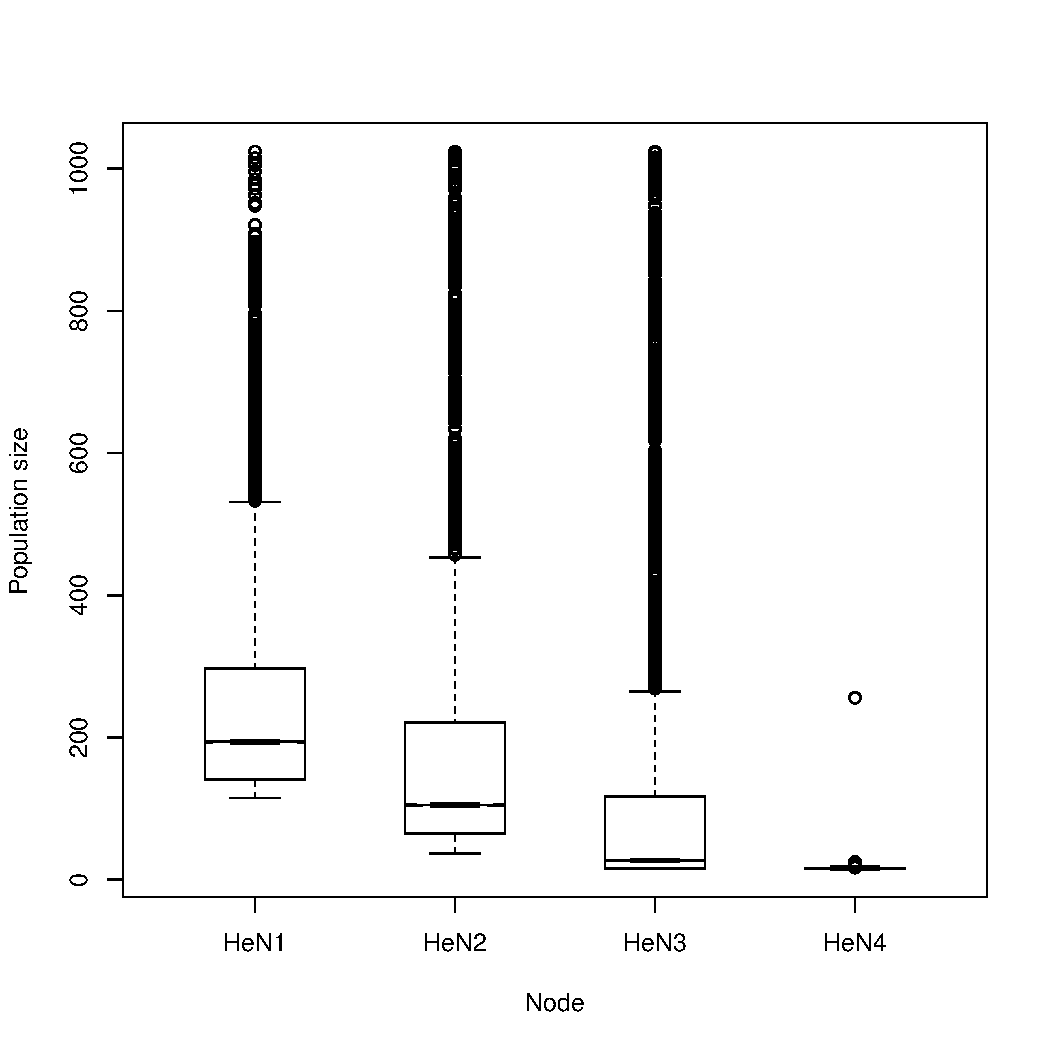
\includegraphics[scale =0.4] {gfx/adaptiveresults/sizesONEMAX.pdf}
\caption{Boxplots of the sub-population sizes in each node during all the runs for the OneMax problem.}
\label{fig:sizesONEMAX}
\end{SCfigure}

\begin{SCfigure}[tb]
\centering
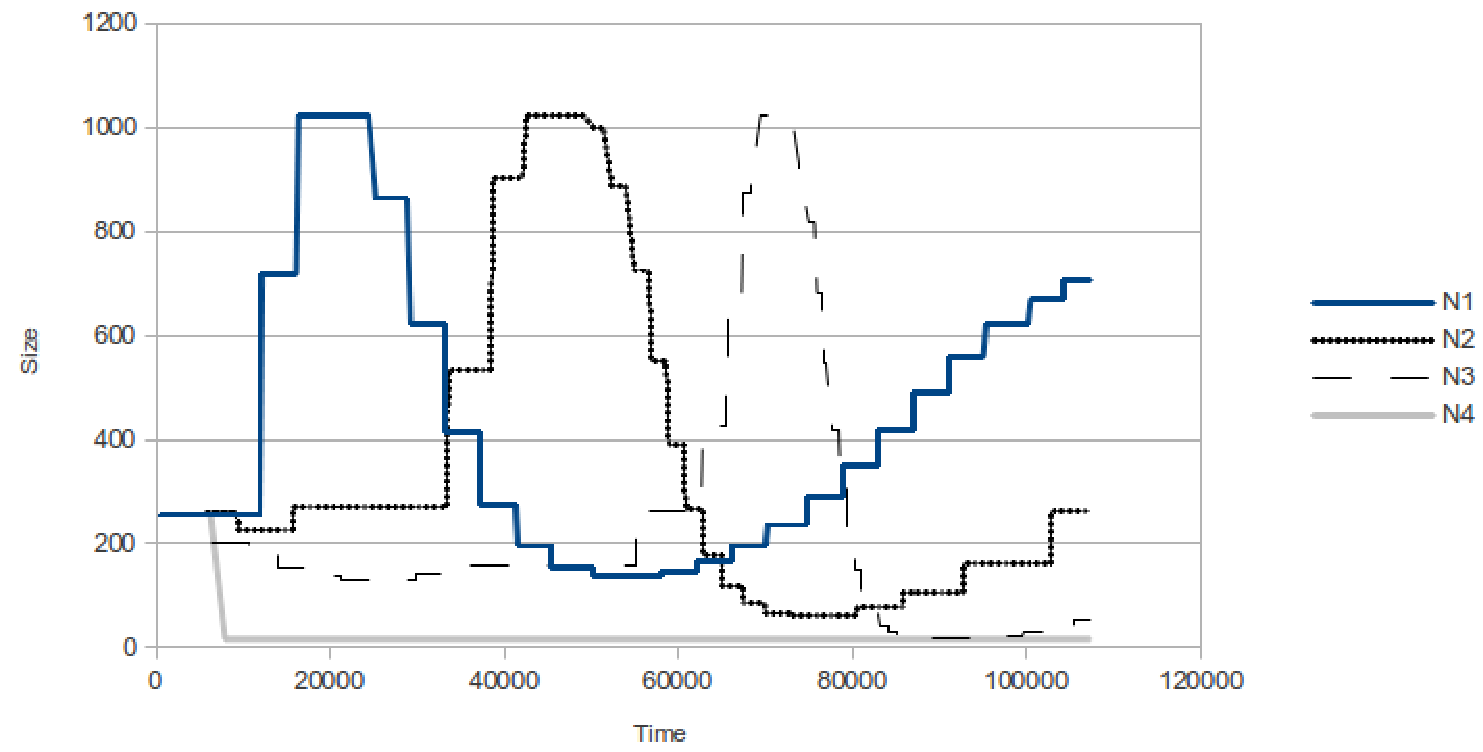
\includegraphics[scale =0.4] {gfx/adaptiveresults/sizesONEMAX1ejec.pdf}
\caption{Sub-population size in each node during one execution to solve the OneMax problem.}
\label{fig:sizesONEMAX1ejec}
\end{SCfigure}


\begin{SCtable}[][tb]
\resizebox{6cm}{!}{
\begin{tabular}{ccccc}
\hline
\rowcolor{colorCorporativoSuave}Node        & HeN1     & HeN2      & HeN3     & HeN4   \\ \hline \hline
\rowcolor{colorCorporativoMasSuave}Size &   267.09 & 158.63 &  74.20  & 16.29 \\ \hline
\rowcolor{colorCorporativoSuave}Proportion  &  51.73 &  30.72 &   14.37 &  3.15  \\ \hline
\end{tabular}
\caption{Average sub-population size in each node on the heterogeneous cluster with adaptive size (OneMax).}
\label{table:sizesONEMAX}
}
\end{SCtable}



\begin{SCtable}[][tb]
\resizebox{11cm}{!}{
\begin{tabular}{cccccc}
\hline

\multicolumn{6}{>{\columncolor{colorCorporativoSuave}}c}{Time} \\ \hline \hline
\multicolumn{6}{>{\columncolor{colorCorporativoMasSuave}}c}{Kruskal-Wallis chi-squared = 20.3042, df = 2, p-value = 3.899e-05} \\ \hline
\rowcolor{colorCorporativoSuave}Configuration       & Test  & obs.dif   & critical.dif  & p-value & difference \\ \hline
\rowcolor{colorCorporativoMasSuave}AdSi/HeHa-HeSi/HeHa      & K-W   & 13.19231  &    18.38851   & 0.1390  &  FALSE \\ \hline
\rowcolor{colorCorporativoSuave}AdSi/HeHa-HoSi/HeHa      & K-W   & 21.11538  &    18.38851   & 0.0067  & TRUE \\ \hline
\rowcolor{colorCorporativoMasSuave}HeSi/HeHa-HoSi/HeHa & K-W   & 34.30769  &    18.38851   & 9\e{-5} & TRUE \\ \hline \hline
\rowcolor{colorCorporativoSuave}HoSi/HoHa-HeSi/HoHa & Wilcoxon & -      & -             & 0.52    & FALSE \\ \hline \hline


\multicolumn{6}{>{\columncolor{colorCorporativoMasSuave}}c}{Evaluations}  \\ \hline \hline
\multicolumn{6}{>{\columncolor{colorCorporativoSuave}}c}{Kruskal-Wallis chi-squared = 11.9676, df = 2, p-value = 0.002519} \\ \hline
\rowcolor{colorCorporativoMasSuave}AdSi/HeHa-HeSi/HeHa      & K-W  & 2.794872   & 18.38851      &  1.0          & FALSE \\ \hline
\rowcolor{colorCorporativoSuave}AdSi/HeHa-HoSi/HeHa      & K-W  & 21.487179  & 18.38851      &  0.0207        & TRUE\\ \hline
\rowcolor{colorCorporativoMasSuave}HeSi/HeHa-HoSi/HeHa & K-W  & 24.282051  & 18.38851      &  0.0028        & TRUE \\ \hline \hline
\rowcolor{colorCorporativoSuave}HoSi/HoHa-HeSi/HoHa &Wilcoxon & -       & -             & 0.08           & FALSE \\ \hline 

\end{tabular}
}
\caption{Statistical significance of the results for MMDP.}
\label{tab:significanceMMDP}
\end{SCtable}


\begin{SCtable}[][tb]
\resizebox{11cm}{!}{
\begin{tabular}{ccccccc}
\hline
\multicolumn{6}{>{\columncolor{colorCorporativoSuave}}c}{Time} \\ \hline \hline
\multicolumn{6}{>{\columncolor{colorCorporativoMasSuave}}c}{Kruskal-Wallis chi-squared = 66.4965, df = 2, p-value = 3.635e-15} \\ \hline
\rowcolor{colorCorporativoSuave}Configuration       & Test  & obs.dif   & critical.dif  & p-value & difference \\ \hline
\rowcolor{colorCorporativoMasSuave}AdSi/HeHa-HeSi/HeHa      & K-W   &  33.27586 &    15.87987   & 2.3\e{-10}  &  TRUE \\ \hline
\rowcolor{colorCorporativoSuave}AdSi/HeHa-HoSi/HeHa      & K-W   &  53.56897 &   15.87987  & $<$2\e{-16}  & TRUE \\ \hline
\rowcolor{colorCorporativoMasSuave}HeSi/HeHa-HoSi/HeHa & K-W   &   20.29310&   15.87987  & 4.2\e{-6}  & TRUE \\ \hline \hline
\rowcolor{colorCorporativoSuave}HoSi/HoHa-HeSi/HoHa & Wilcoxon & -      & -             & 3\e{-8}   & TRUE \\ \hline \hline


\multicolumn{6}{>{\columncolor{colorCorporativoMasSuave}}c}{Evaluations}  \\ \hline \hline
\multicolumn{6}{>{\columncolor{colorCorporativoSuave}}c}{Kruskal-Wallis chi-squared = 75.7342, df = 2, p-value $<$ 2.2e-16} \\ \hline
\rowcolor{colorCorporativoMasSuave}AdSi/HeHa-HeSi/HeHa      & K-W  &  57.72414   &  15.87987     & $<$2\e{-16}          & TRUE \\ \hline
\rowcolor{colorCorporativoSuave}AdSi/HeHa-HoSi/HeHa      & K-W  &  29.27586   &   15.87987    & $<$2\e{-16}         & TRUE\\ \hline
\rowcolor{colorCorporativoMasSuave}HeSi/HeHa-HoSi/HeHa & K-W  &  28.44828   &  15.87987     &  $<$1.3\e{-14}        & TRUE \\ \hline \hline
\rowcolor{colorCorporativoSuave}HoSi/HoHa-HeSi/HoHa &Wilcoxon & -       & -              &  3\e{-8}          & TRUE \\ \hline 

\end{tabular}
}
\caption{Statistical significance of the results for OneMax.}
\label{tab:significanceONEMAX}
\end{SCtable}


% OMG páginas y páginas de tablas y gráficos - JJ

\subsection{Running time analysis}

This sub-section shows the analysis the time spent by each node of the clusters
in every %¿lo haces tú o la subsección? - JJ FERGU: cambiado
 service of the EA for each configuration with fixed sizes (HoSi and HeSi). Tables \ref{tab:mmdptimes} and \ref{tab:onemaxtimes} show the average and standard deviation of the time spent in each stage of the algorithm (He=Heterogeneous cluster, Ho=Homogeneous cluster). Figures \ref{fig:MMDPbars} and \ref{fig:ONEMAXbars} graphically compare these results. As it can be seen, the migration is the most time consuming operation in all configurations, being the migration in HeHa more expensive than in HoHa. This happens because we are using the multi-purpose laboratory network to communicate the nodes, instead of the specific one used in the HoHa system. Note that the standard deviation of the migration is larger in the HeHa cluster because the network is having real conditions of traffic during the experiment. In the MMDP problem (Table \ref{tab:mmdptimes}) changing the sub-population size does not affect the migration time, but it affects the rest of the algorithm's stages. However, with larger data communications (individuals of 5000 elements of the OneMax problem), the sub-population size affects the migration time of all nodes. This might be due to the synchronization of migration buffers: if the slowest machine is sending/receiving, bottlenecks can be propagated (as it can be seen in Figure \ref{fig:gensonemaxhomosize}). 

Results also show how the stages of the algorithms depends on the node
of execution. For example, recombination needs more time than mutation
in both problems only in the node HeN4. The reason might be the
creation of new objects (memory allocation), which in Java and in
% en una tesis no se puede decir "might be". Diseñas un experimento
% para probar si esto es cierto o no. Y "diseñas un experimento"
% quiere decir que lo hagas y lo añadas al capítulo - JJ
limited memory (and swapping) requires more time than the iteration of
elements previously created (for example, in the mutation). Adapting
the sub-population size makes the slower node of HeHa behave in similar
way than the other nodes (same time in each stage). Moreover, the size
of the individuals affects to some parts of the EA; for example, in 
OneMax the mutation requires more time than the replacement. However,
it must be taken into account that the duration of each part of the
algorithm is not related to the time to attain the optimum, but rather to
how the diversity and search guidance is maintained in the whole system.  

\begin{SCfigure}[tb]
\centering
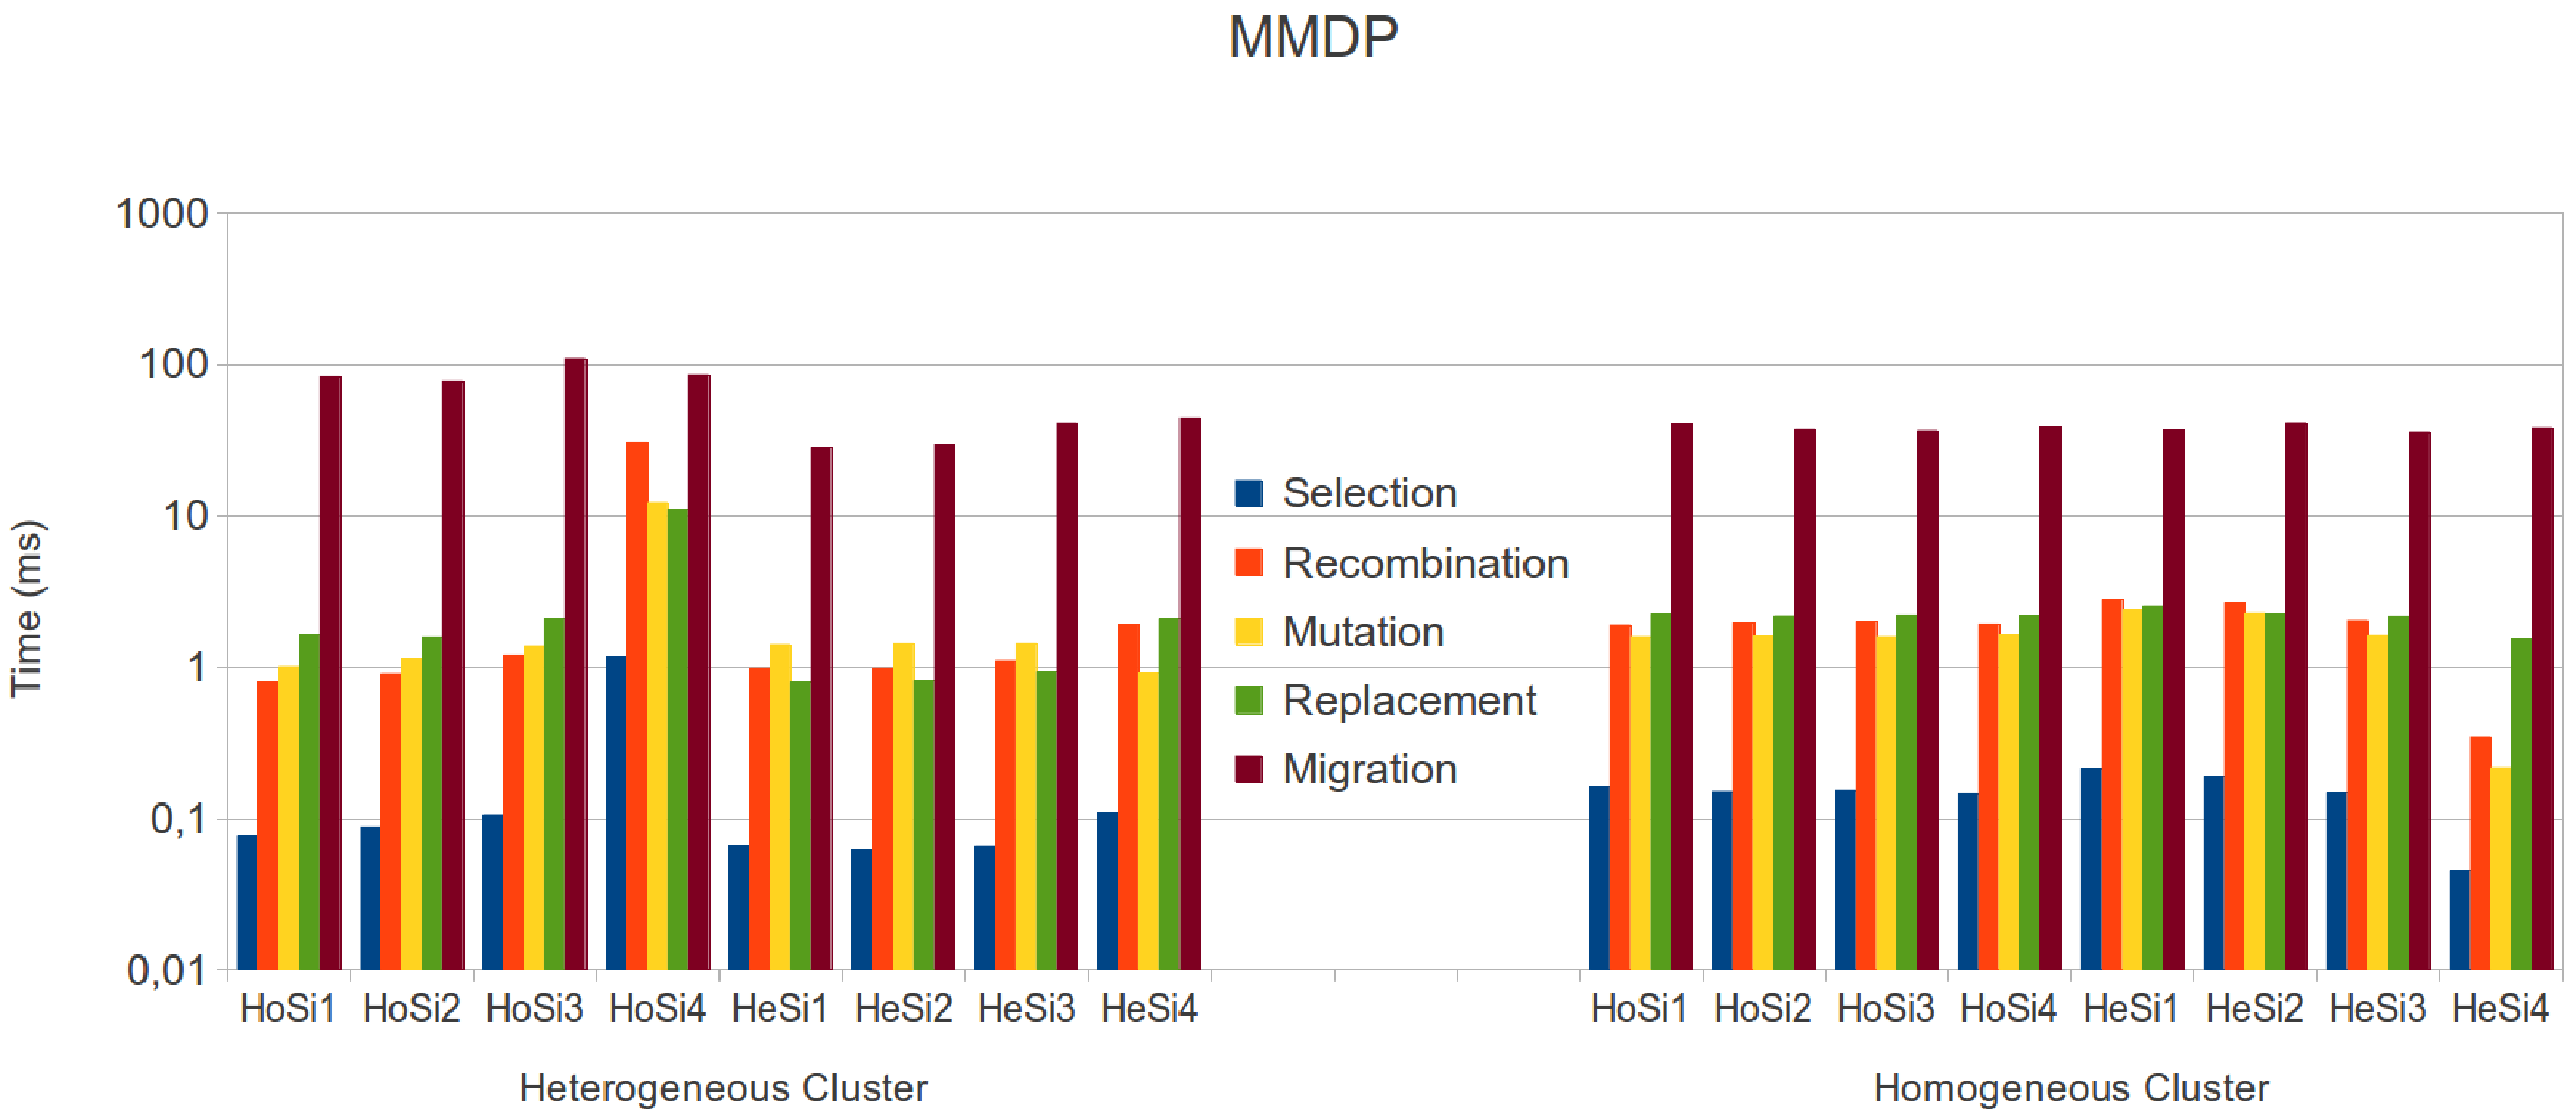
\includegraphics[scale =0.19] {gfx/adaptiveresults/timingMMDP.pdf}
\caption{Average running time in each stage of the algorithm for the MMDP problem.}
\label{fig:MMDPbars}
\end{SCfigure}

\begin{SCfigure}[tb]
\centering
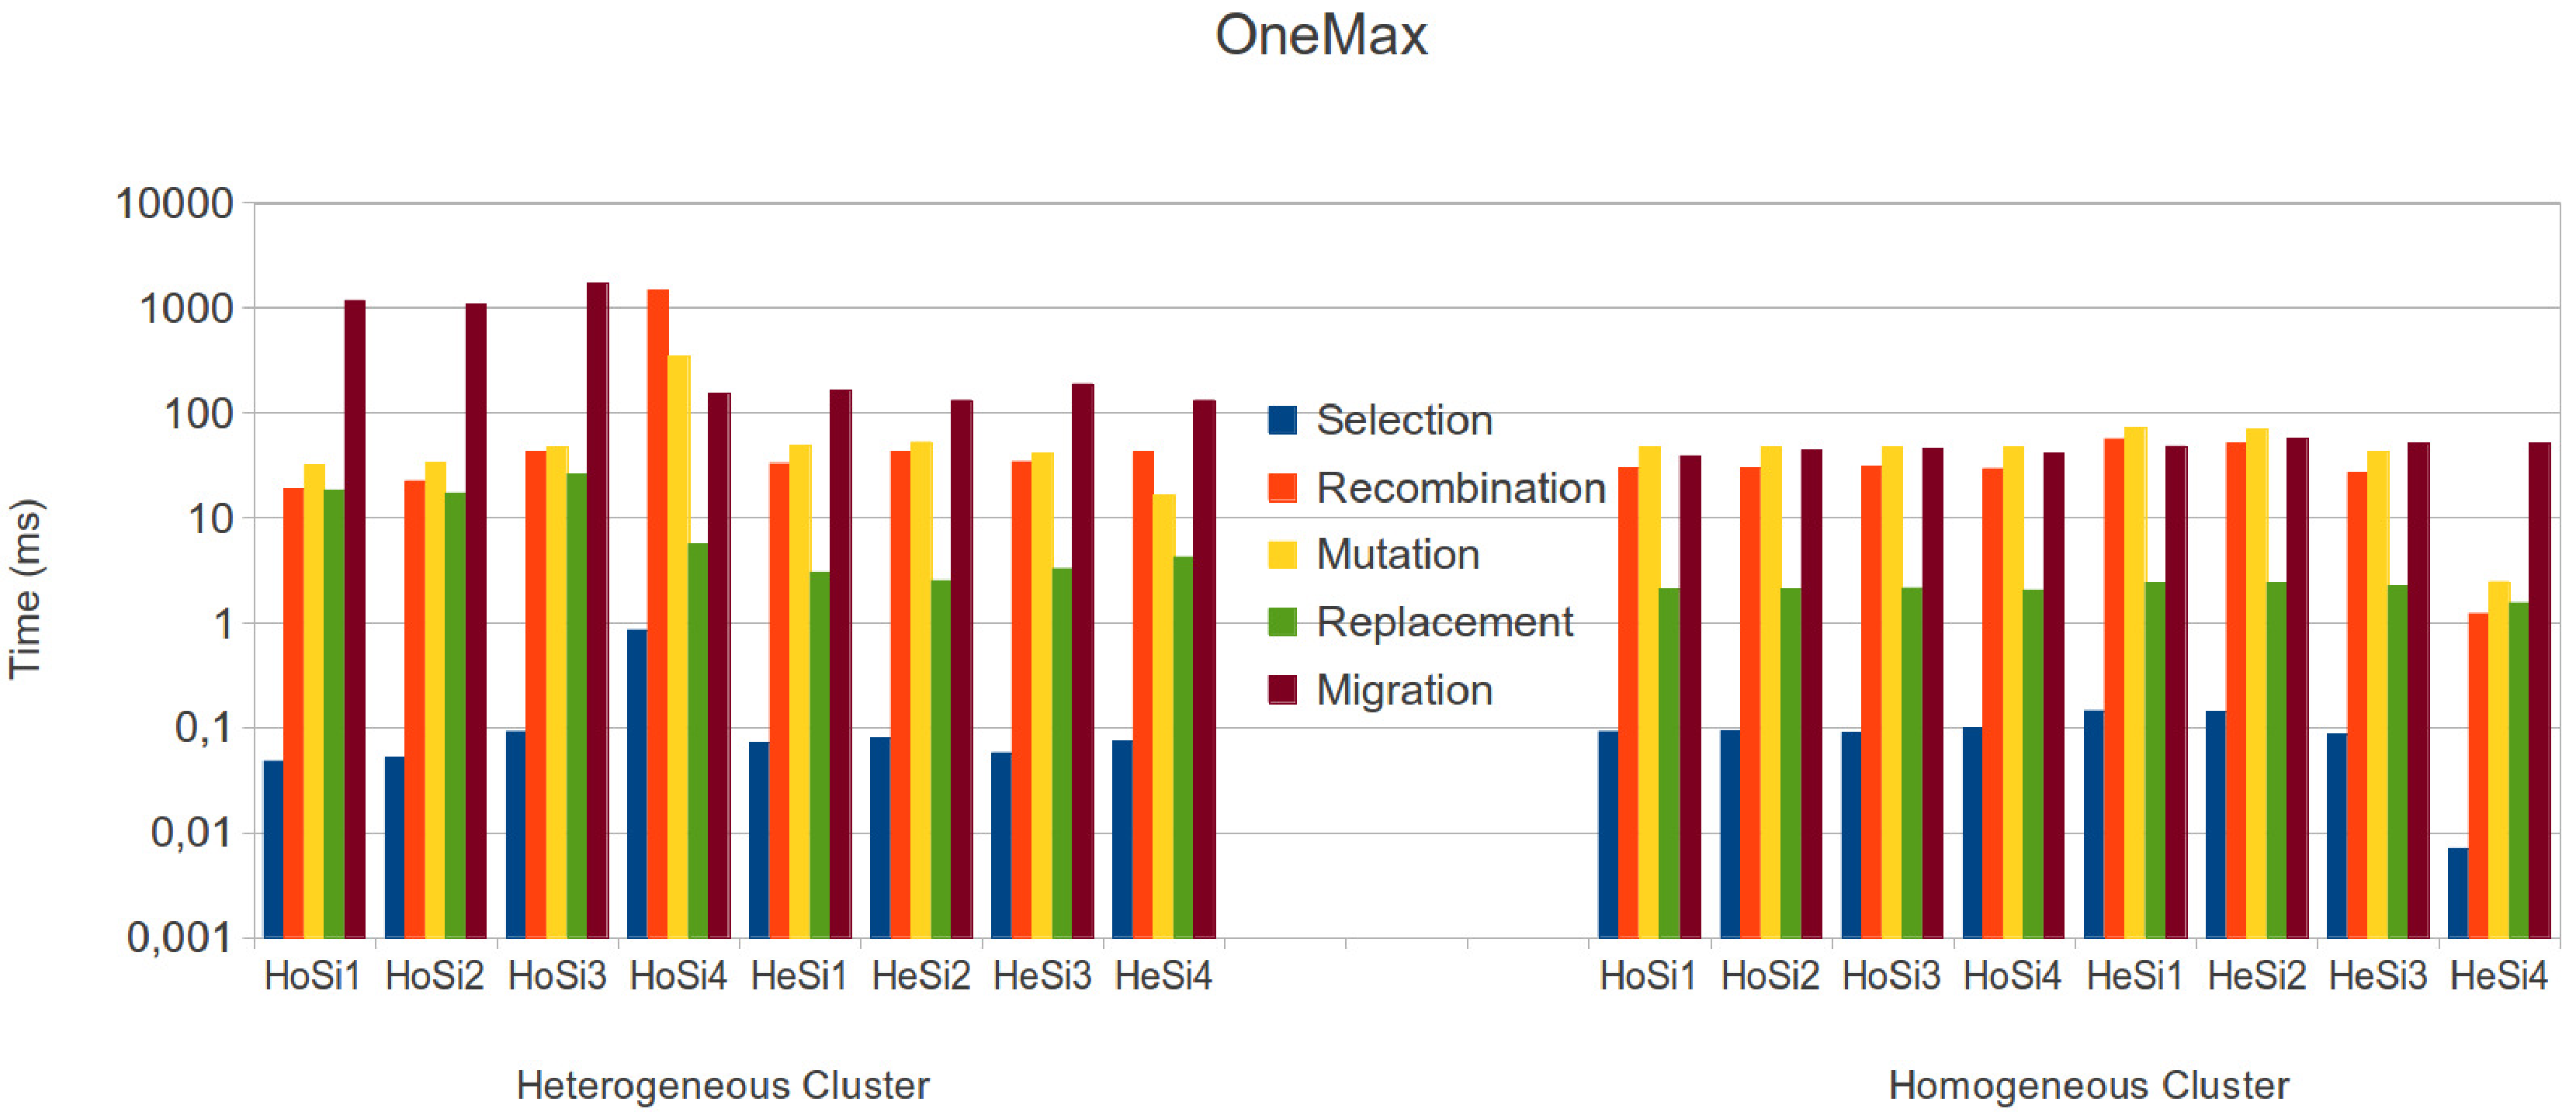
\includegraphics[scale =0.19] {gfx/adaptiveresults/timingONEMAX.pdf}
\caption{Average running time in each stage of the algorithm for the ONEMAX problem.}
\label{fig:ONEMAXbars}
\end{SCfigure}

\begin{SCtable}[][tb]
\resizebox{11cm}{!}{
\begin{tabular}{ccccccc}
\hline
\multicolumn{6}{>{\columncolor{colorCorporativoSuave}}c}{Heterogeneous Cluster} \\ \hline \hline
\rowcolor{colorCorporativoMasSuave}Node    & Selection     & Recombination     & Mutation      & Replacement       & Migration         \\ \hline
\rowcolor{colorCorporativoSuave}HoSi HeN1    & 0.077 $\pm$  0.170 &  0.788  $\pm$ 0.779  & 1.004  $\pm$ 0.187 &  1.648  $\pm$ 20.185 & 82.458  $\pm$ 143.266 \\ \hline
\rowcolor{colorCorporativoMasSuave}HoSi HeN2    & 0.088 $\pm$  0.190 &  0.907 $\pm$  0.932  & 1.145  $\pm$ 0.425 &  1.579  $\pm$ 17.907 & 76.725  $\pm$ 126.360\\ \hline
\rowcolor{colorCorporativoSuave}HoSi HeN3    & 0.105 $\pm$  0.163 &  1.207 $\pm$  0.927  & 1.374  $\pm$ 0.301 &  2.108  $\pm$ 21.848 & 108.605 $\pm$ 142.633\\ \hline
\rowcolor{colorCorporativoMasSuave}HoSi HeN4    & 1.165 $\pm$  1.526 &  30.445$\pm$  59.553 & 12.221 $\pm$ 7.412 &  10.978 $\pm$ 57.135 & 84.936  $\pm$ 0.000\\ \hline \hline
\rowcolor{colorCorporativoSuave}HeSi HeN1    & 0.067 $\pm$  0.065  & 0.973  $\pm$ 0.403 &  1.411 $\pm$  0.166 &  0.790  $\pm$ 6.266 &  28.081 $\pm$ 42.169 \\ \hline
\rowcolor{colorCorporativoMasSuave}HeSi HeN2    & 0.062 $\pm$  0.075  & 0.973  $\pm$ 0.470 &  1.433 $\pm$  0.265 &  0.811  $\pm$ 7.056 &  29.667 $\pm$ 48.702 \\ \hline
\rowcolor{colorCorporativoSuave}HeSi HeN3    & 0.066 $\pm$  0.108  & 1.104  $\pm$ 0.346 &  1.435 $\pm$  0.296 &  0.937  $\pm$ 7.072 &  40.964 $\pm$ 40.027 \\ \hline
\rowcolor{colorCorporativoMasSuave}HeSi HeN4    & 0.109 $\pm$  0.257  & 1.895  $\pm$ 5.611 &  0.913 $\pm$  0.834 &  2.085  $\pm$ 5.626 &  43.880 $\pm$ 7.535 \\ \hline 

\hline \hline
\multicolumn{6}{>{\columncolor{colorCorporativoSuave}}c}{Homogeneous Cluster} \\ \hline  \hline                               
\rowcolor{colorCorporativoMasSuave}Node    & Selection     & Recombination     & Mutation      & Replacement       & Migration \\ \hline
\rowcolor{colorCorporativoSuave}HoSi HoN1    & 0.163 $\pm$  0.223 &  1.884 $\pm$  2.386  & 1.591  $\pm$ 0.479 &  2.254  $\pm$ 5.513  & 40.256  $\pm$ 8.726\\ \hline
\rowcolor{colorCorporativoMasSuave}HoSi HoN2    & 0.151 $\pm$  0.212 &  1.952 $\pm$  2.876  & 1.597  $\pm$ 0.574 &  2.178  $\pm$ 4.922  & 37.110  $\pm$ 6.999\\ \hline
\rowcolor{colorCorporativoSuave}HoSi HoN3    & 0.154 $\pm$  0.206 &  1.990 $\pm$  3.010  & 1.591  $\pm$ 0.577 &  2.215  $\pm$ 4.743  & 36.413  $\pm$ 5.266\\ \hline
\rowcolor{colorCorporativoMasSuave}HoSi HoN4    & 0.146 $\pm$  0.196 &  1.913 $\pm$  2.697  & 1.651  $\pm$ 1.167 &  2.194  $\pm$ 5.124  & 38.429  $\pm$ 6.192\\ \hline \hline
\rowcolor{colorCorporativoSuave}HeSi HoN1    & 0.214 $\pm$  0.288  & 2.800  $\pm$ 3.793 &  2.359 $\pm$  0.691 &  2.516  $\pm$ 4.706 &  36.972 $\pm$ 4.214 \\ \hline
\rowcolor{colorCorporativoMasSuave}HeSi HoN2    & 0.190 $\pm$  0.252  & 2.672  $\pm$ 3.902 &  2.277 $\pm$  0.649 &  2.261  $\pm$ 4.546 &  41.171 $\pm$ 9.672 \\ \hline
\rowcolor{colorCorporativoSuave}HeSi HoN3    & 0.148 $\pm$  0.208  & 2.030  $\pm$ 3.161 &  1.623 $\pm$  0.500 &  2.164  $\pm$ 4.512 &  35.551 $\pm$  6.132 \\ \hline
\rowcolor{colorCorporativoMasSuave}HeSi HoN4    & 0.045 $\pm$  0.052  & 0.345  $\pm$ 1.121 &  0.217 $\pm$  0.142 &  1.531  $\pm$ 4.856 &  38.106 $\pm$ 9.251 \\ \hline
\end{tabular}
}
\caption{Times of the stages of the algorithm for the MMDP problem (in ms).}
\label{tab:mmdptimes}
\end{SCtable}








\begin{SCtable}[][tb]
\resizebox{11cm}{!}{
\begin{tabular}{ccccccc}
\hline
\multicolumn{6}{>{\columncolor{colorCorporativoSuave}}c}{Heterogeneous Cluster} \\ \hline \hline
\rowcolor{colorCorporativoMasSuave}Node    & Selection     & Recombination     & Mutation      & Replacement       & Migration         \\ \hline
\rowcolor{colorCorporativoSuave}HoSi HeN1  &  0.048 $\pm$  0.043  & 18.713 $\pm$ 13.454 & 31.984 $\pm$ 2.104  & 18.375 $\pm$ 197.676 & 1172.986  $\pm$  1108.388 \\ \hline
\rowcolor{colorCorporativoMasSuave}HoSi HeN2  &  0.052 $\pm$  0.051  & 22.266 $\pm$  22.716 & 33.553 $\pm$ 4.931 &  17.176 $\pm$ 180.580 & 1085.508  $\pm$  995.382 \\ \hline
\rowcolor{colorCorporativoSuave}HoSi HeN3  &  0.091 $\pm$  1.005  & 42.634 $\pm$ 21.621  & 47.674 $\pm$ 0.546 &  26.094 $\pm$ 252.667 & 1708.402 $\pm$   1207.925 \\ \hline
\rowcolor{colorCorporativoMasSuave}HoSi HeN4  &  0.851  $\pm$ 0.435  & 1491.568 $\pm$ 1185.723 & 344.872$\pm$ 6.634 &  5.655  $\pm$ 16.175 & 154.019 $\pm$0.000 \\ \hline \hline
\rowcolor{colorCorporativoSuave}HeSi HeN1 &   0.072 $\pm$  0.063 &  32.917 $\pm$ 26.792 & 49.103 $\pm$ 2.655  & 3.023 $\pm$  27.647 & 163.479 $\pm$157.172 \\ \hline
\rowcolor{colorCorporativoMasSuave}HeSi HeN2 &   0.080 $\pm$  0.092 &  43.001 $\pm$ 51.680 & 52.288 $\pm$ 13.210 & 2.527 $\pm$  21.861 & 131.063 $\pm$124.404 \\ \hline
\rowcolor{colorCorporativoSuave}HeSi HeN3 &   0.057 $\pm$  0.052 &  33.951 $\pm$ 15.063 & 41.375 $\pm$ 1.707  & 3.284 $\pm$  30.170 & 186.467 $\pm$163.906 \\ \hline
\rowcolor{colorCorporativoMasSuave}HeSi HeN4 &   0.075 $\pm$  0.107 &  42.443 $\pm$ 88.536 & 16.236 $\pm$ 12.028 & 4.194 $\pm$  33.119 & 131.135 $\pm$144.359 \\ \hline 

\hline \hline
\multicolumn{6}{>{\columncolor{colorCorporativoSuave}}c}{Homogeneous Cluster} \\ \hline  \hline                               
\rowcolor{colorCorporativoMasSuave}Node    & Selection     & Recombination     & Mutation      & Replacement       & Migration \\ \hline
\rowcolor{colorCorporativoSuave}HoSi HoN1  &  0.091 $\pm$  0.078  & 29.969 $\pm$ 21.459 & 47.445 $\pm$ 2.194 &  2.073 $\pm$  6.970 &  38.782 $\pm$ 40.369 \\ \hline
\rowcolor{colorCorporativoMasSuave}HoSi HoN2  &  0.093 $\pm$  0.082  & 30.119 $\pm$ 22.029 & 47.247 $\pm$ 2.146 &  2.108 $\pm$  7.440 &  44.303 $\pm$ 42.759 \\ \hline
\rowcolor{colorCorporativoSuave}HoSi HoN3  &  0.089 $\pm$  0.080  & 30.951 $\pm$ 21.904 & 47.103 $\pm$ 2.031 &  2.138 $\pm$  8.006 &  46.107 $\pm$ 47.351 \\ \hline
\rowcolor{colorCorporativoMasSuave}HoSi HoN4  &  0.098 $\pm$  0.075  & 29.468 $\pm$ 20.876 & 47.086 $\pm$ 1.856 &  2.043 $\pm$  7.491 &  41.458 $\pm$ 44.970 \\ \hline \hline
\rowcolor{colorCorporativoSuave}HeSi HoN1 &   0.144 $\pm$  0.151 &  56.124 $\pm$ 48.229 & 72.811 $\pm$ 5.177  & 2.424 $\pm$  9.056  & 48.165  $\pm$57.798 \\ \hline
\rowcolor{colorCorporativoMasSuave}HeSi HoN2 &   0.141 $\pm$  0.152 &  51.226 $\pm$ 41.016 & 70.047 $\pm$ 4.152  & 2.427 $\pm$  10.890 & 57.152  $\pm$74.177 \\ \hline
\rowcolor{colorCorporativoSuave}HeSi HoN3 &   0.086 $\pm$  0.088 &  26.932 $\pm$ 20.460 & 42.963 $\pm$ 3.935  & 2.239 $\pm$  8.658  & 51.014  $\pm$49.648 \\ \hline
\rowcolor{colorCorporativoMasSuave}HeSi HoN4 &   0.007 $\pm$  0.008 &  1.215  $\pm$ 1.133  & 2.470  $\pm$ 0.098  & 1.553 $\pm$  10.078 & 50.498 $\pm$ 63.983 \\ \hline
\end{tabular}
}
\caption{Times of the stages of the algorithm for the OneMax problem (in ms).}
\label{tab:onemaxtimes}
\end{SCtable}

%AGH! No hay conclusión. ¿Cómo avanza esto la tesis? ¿Qué relación
%tiene con el capítulo siguiente? Todos los capítulos deben tener una
%introducción, una línea argumental y una conclusión - JJ FERGU: es que lo revisaste antes de terminarlo :P (añadidas las conclusiones)

\section{Conclusions}



% No. Tratamos de
                                % probar un objetivo, dilo aquí!!!!!

%Results show that adapting (online or offline) the population size to the computational power of each node in the heterogeneous cluster yields significantly
%better results in time than keeping the same parameter in all
%nodes. This advantage is due to the combination of the heterogeneous
%parameters with the heterogeneity of the machines. % o sea, tener
                                % maquinas heterogéneas y parámetros
                                % heterogéneos es mejor porque usamos
                                % parámetros heterogéneos en máquinas
                                % heterogéneas. Di en qué puede
                                % influir eso en la mejora de los
                                % resultados y discute por qué podría
                                % ser así y propón experimentos para
                                % probar que efectivamente se trata de
                                % eso. - JJ
%On the contrary,
%the same (heterogeneous) parameter setting in all islands of the
%homogeneous cluster could not improve the results than considering the
%same parameter value in all nodes. % ¿Y qué más da?  ¿Por qué es esto
                                % relevante? Di que, por tanto, la
                                % mejora no se debe al cambio de
                                % parámetros sólo, sino a la
                                % combinación entre cambio de
                                % parámetros y adaptación al nodo - JJ 

In this chapter, OSGiLiath has been used to present a study on the adaptation of the sub-population sizes of a distributed EA to the computational power of the different nodes of an heterogeneous cluster.  Different services for migration and algorithm control have been created to be automatically bound. Two adaptation schemes (offline and online) that use information of the computational load of the algorithm have been tested.

Results show that adapting (online or offline) the sub-population size to the computational power of each node in the heterogeneous cluster yields significantly
better results in time than keeping the same parameter in all nodes. This advantage is due to the combination of the heterogeneous parameters with the heterogeneity of the machines. On the contrary, the same (heterogeneous) parameter setting in all islands of the homogeneous cluster could not improve the results than considering the same parameter value in all nodes.



Furthermore, changing the sub-population size affects to stages
of the algorithm that are independent of this parameter, such as
the migration. The sub-population size adaptation is also affected by the problem to solve.

In this chapter, as a possible offline parameter setting, we have calculated the computational power of each node proportionally 
to the average number of generations of the homogeneous parameter set. Moreover, a possible way to adapt 
online the sub-population sizes has been performed comparing the current generation with
 the neighbour generation. These results are a promising starting for adapting EAs to the
performance of each execution node with OSGiLiath, using more adequate benchmarks or in a dynamic way. 
% Falta una discusión sobre si las mejoras se deben exclusivamente al
% número de evaluaciones o hay algún otro factor ¿menos overhead?
% ¿nodos más rápidos? - JJ FERGU: no, de hecho el número de evaluaciones no siempre disminuye, lo digo arriba.

In the future it would be interesting to check the scalability of this
approach, using more computational nodes and larger problem
instances. In addition, other parameters such as migration rate or
crossover probability could be adapted to the execution
nodes. Different implementation of these services could be automatically enabled depending of the current state of the EA and the node. 
Other appropriate benchmark services to analyse the algorithm will be also used to lead to automatic
parameter adaptation in runtime (online), with different nodes entering or
exiting in the topology, or adapting the parameters to the current load of the
system. 

